% Options for packages loaded elsewhere
\PassOptionsToPackage{unicode}{hyperref}
\PassOptionsToPackage{hyphens}{url}
\PassOptionsToPackage{dvipsnames,svgnames,x11names}{xcolor}
%
\documentclass[
  letterpaper,
  DIV=11,
  numbers=noendperiod]{scrartcl}

\usepackage{amsmath,amssymb}
\usepackage{iftex}
\ifPDFTeX
  \usepackage[T1]{fontenc}
  \usepackage[utf8]{inputenc}
  \usepackage{textcomp} % provide euro and other symbols
\else % if luatex or xetex
  \usepackage{unicode-math}
  \defaultfontfeatures{Scale=MatchLowercase}
  \defaultfontfeatures[\rmfamily]{Ligatures=TeX,Scale=1}
\fi
\usepackage{lmodern}
\ifPDFTeX\else  
    % xetex/luatex font selection
\fi
% Use upquote if available, for straight quotes in verbatim environments
\IfFileExists{upquote.sty}{\usepackage{upquote}}{}
\IfFileExists{microtype.sty}{% use microtype if available
  \usepackage[]{microtype}
  \UseMicrotypeSet[protrusion]{basicmath} % disable protrusion for tt fonts
}{}
\makeatletter
\@ifundefined{KOMAClassName}{% if non-KOMA class
  \IfFileExists{parskip.sty}{%
    \usepackage{parskip}
  }{% else
    \setlength{\parindent}{0pt}
    \setlength{\parskip}{6pt plus 2pt minus 1pt}}
}{% if KOMA class
  \KOMAoptions{parskip=half}}
\makeatother
\usepackage{xcolor}
\setlength{\emergencystretch}{3em} % prevent overfull lines
\setcounter{secnumdepth}{5}
% Make \paragraph and \subparagraph free-standing
\ifx\paragraph\undefined\else
  \let\oldparagraph\paragraph
  \renewcommand{\paragraph}[1]{\oldparagraph{#1}\mbox{}}
\fi
\ifx\subparagraph\undefined\else
  \let\oldsubparagraph\subparagraph
  \renewcommand{\subparagraph}[1]{\oldsubparagraph{#1}\mbox{}}
\fi


\providecommand{\tightlist}{%
  \setlength{\itemsep}{0pt}\setlength{\parskip}{0pt}}\usepackage{longtable,booktabs,array}
\usepackage{calc} % for calculating minipage widths
% Correct order of tables after \paragraph or \subparagraph
\usepackage{etoolbox}
\makeatletter
\patchcmd\longtable{\par}{\if@noskipsec\mbox{}\fi\par}{}{}
\makeatother
% Allow footnotes in longtable head/foot
\IfFileExists{footnotehyper.sty}{\usepackage{footnotehyper}}{\usepackage{footnote}}
\makesavenoteenv{longtable}
\usepackage{graphicx}
\makeatletter
\def\maxwidth{\ifdim\Gin@nat@width>\linewidth\linewidth\else\Gin@nat@width\fi}
\def\maxheight{\ifdim\Gin@nat@height>\textheight\textheight\else\Gin@nat@height\fi}
\makeatother
% Scale images if necessary, so that they will not overflow the page
% margins by default, and it is still possible to overwrite the defaults
% using explicit options in \includegraphics[width, height, ...]{}
\setkeys{Gin}{width=\maxwidth,height=\maxheight,keepaspectratio}
% Set default figure placement to htbp
\makeatletter
\def\fps@figure{htbp}
\makeatother
% definitions for citeproc citations
\NewDocumentCommand\citeproctext{}{}
\NewDocumentCommand\citeproc{mm}{%
  \begingroup\def\citeproctext{#2}\cite{#1}\endgroup}
\makeatletter
 % allow citations to break across lines
 \let\@cite@ofmt\@firstofone
 % avoid brackets around text for \cite:
 \def\@biblabel#1{}
 \def\@cite#1#2{{#1\if@tempswa , #2\fi}}
\makeatother
\newlength{\cslhangindent}
\setlength{\cslhangindent}{1.5em}
\newlength{\csllabelwidth}
\setlength{\csllabelwidth}{3em}
\newenvironment{CSLReferences}[2] % #1 hanging-indent, #2 entry-spacing
 {\begin{list}{}{%
  \setlength{\itemindent}{0pt}
  \setlength{\leftmargin}{0pt}
  \setlength{\parsep}{0pt}
  % turn on hanging indent if param 1 is 1
  \ifodd #1
   \setlength{\leftmargin}{\cslhangindent}
   \setlength{\itemindent}{-1\cslhangindent}
  \fi
  % set entry spacing
  \setlength{\itemsep}{#2\baselineskip}}}
 {\end{list}}
\usepackage{calc}
\newcommand{\CSLBlock}[1]{\hfill\break\parbox[t]{\linewidth}{\strut\ignorespaces#1\strut}}
\newcommand{\CSLLeftMargin}[1]{\parbox[t]{\csllabelwidth}{\strut#1\strut}}
\newcommand{\CSLRightInline}[1]{\parbox[t]{\linewidth - \csllabelwidth}{\strut#1\strut}}
\newcommand{\CSLIndent}[1]{\hspace{\cslhangindent}#1}

\KOMAoption{captions}{tableheading}
\makeatletter
\@ifpackageloaded{caption}{}{\usepackage{caption}}
\AtBeginDocument{%
\ifdefined\contentsname
  \renewcommand*\contentsname{Table of contents}
\else
  \newcommand\contentsname{Table of contents}
\fi
\ifdefined\listfigurename
  \renewcommand*\listfigurename{List of Figures}
\else
  \newcommand\listfigurename{List of Figures}
\fi
\ifdefined\listtablename
  \renewcommand*\listtablename{List of Tables}
\else
  \newcommand\listtablename{List of Tables}
\fi
\ifdefined\figurename
  \renewcommand*\figurename{Figure}
\else
  \newcommand\figurename{Figure}
\fi
\ifdefined\tablename
  \renewcommand*\tablename{Table}
\else
  \newcommand\tablename{Table}
\fi
}
\@ifpackageloaded{float}{}{\usepackage{float}}
\floatstyle{ruled}
\@ifundefined{c@chapter}{\newfloat{codelisting}{h}{lop}}{\newfloat{codelisting}{h}{lop}[chapter]}
\floatname{codelisting}{Listing}
\newcommand*\listoflistings{\listof{codelisting}{List of Listings}}
\makeatother
\makeatletter
\makeatother
\makeatletter
\@ifpackageloaded{caption}{}{\usepackage{caption}}
\@ifpackageloaded{subcaption}{}{\usepackage{subcaption}}
\makeatother
\ifLuaTeX
  \usepackage{selnolig}  % disable illegal ligatures
\fi
\usepackage{bookmark}

\IfFileExists{xurl.sty}{\usepackage{xurl}}{} % add URL line breaks if available
\urlstyle{same} % disable monospaced font for URLs
\hypersetup{
  pdftitle={Conditional Probability Density Functions},
  pdfauthor={Michael Betancourt},
  colorlinks=true,
  linkcolor={blue},
  filecolor={Maroon},
  citecolor={Blue},
  urlcolor={Blue},
  pdfcreator={LaTeX via pandoc}}

\title{Conditional Probability Density Functions}
\author{Michael Betancourt}
\date{February 2023}

\begin{document}
\maketitle
\begin{abstract}
All probability theory chapters can be found
\href{http://www.symplectomorphic.com/writing/\#part1}{here}.

A repository containing all of the files used to generate this chapter
is available on
\href{https://github.com/betanalpha/quarto_chapters/tree/main/9_conditional_probability_density_functions}{GitHub}.
\end{abstract}

\renewcommand*\contentsname{Table of contents}
{
\hypersetup{linkcolor=}
\setcounter{tocdepth}{3}
\tableofcontents
}
\newcommand{\I}[2]{\mathbb{I}_{#1} \! \left[ #2 \right]}

\newcommand{\E}[2]{\mathbb{E}_{#1} \! \left[ #2 \right]}

\newcommand{\rnd}[2]{\frac{ \mathrm{d} #1}{ \mathrm{d} #2 }}

In the
\href{http://www.symplectomorphic.com/assets/chapters_html/conditional_probability_theory.html}{previous
chapter}, we learned how to use conditional probability theory to
decompose probability distributions across partitions, with a particular
focus on partitions implicitly defined by the level sets of a function.
This construction of conditional probability distributions was
relatively straightforward, if a bit abstract.

In applied practice, however, we typically work with not probability
distributions but rather their probability density function
representations. Unfortunately, rigorously constructing conditional
probability density functions requires additional care. To do so
properly, we will need \emph{all} of the measure theory tools that we
have developed to this point, and a few more that I will introduce
below. Buckle up, and make sure that you are aware of your nearest
emergency exit.

\section{The Utility Of Integral
Notation}\label{the-utility-of-integral-notation}

Before diving into conditional probability density functions, let's take
a second to ponder notation.

Recall that partially evaluating a regular conditional probability
kernel on any \(y \in Y\) yields a conditional probability distribution,
\begin{alignat*}{6}
\pi^{f}_{y} :\; &\mathcal{X}& &\rightarrow& \; &[0, 1]&
\\
&\mathsf{x}& &\mapsto& &\pi^{f}( \mathsf{x} \mid y )&,
\end{alignat*} that completely concentrates on the corresponding level
set \(f^{-1}(y)\). When paired with an integrand
\(g : X \rightarrow \mathbb{R}\), the collection of all conditional
probability distributions then defines a conditional expectation
function, \begin{alignat*}{6}
e_{g} : \; &Y& &\rightarrow& \; &\mathbb{R}&
\\
&y& &\mapsto& & \mathbb{E}_{ \pi^{f}_{y} } \! \left[  g  \right]&.
\end{alignat*} The law of total expectation states that the pushforward
expectation of this conditional expectation function is always equal to
the expectation value with respect to the initial probability
distribution, \[
\mathbb{E}_{\pi} \! \left[ g \right] = \mathbb{E}_{ f_{*} \pi } \! \left[ e_{g} \right].
\]

This statement of the law of total expectation is certainly compact, but
it can be also be hard to read. In particular, nothing in the final
equation denotes the spaces associated with each object.

There are many ways that we might try to make the law of total
expectation more explicit. For instance, we could move away from the
standard expectation notation and introduce arguments to the expectands,
\[
\mathbb{E}_{\pi} \! \left[ g \right]
= \mathbb{E}_{ f_{*} \pi } \! \left[ e_{g}(y)  \right]
= \mathbb{E}_{ f_{*} \pi } \! \left[  \mathbb{E}_{\pi^{f}_{y}} \! \left[ g(x) \right]  \right].
\] That said, the resulting notation is relatively dense and can be even
harder to parse than the initial equation.

One way around these potential frustrations is to use the integral
notation for expectation values that we first discussed in
\href{http://www.symplectomorphic.com/assets/chapters_html/expectation_values.html\#sec:alt_notations}{Chapter
5, Section 2.4}. This notation uses variables to explicitly specify the
spaces on which all of the probability distributions and functions are
defined, but allows enough space for the equations to be more readable.

If we interpret each conditional probability distribution
\(\pi^{f}_{y}\) as a probability distribution defined over the entirely
of the ambient space \(X\), then the conditional expectation function
can be written as \begin{align*}
e_{g}(y)
&=
\mathbb{E}_{ \pi^{f}_{y} } \! \left[  g  \right]
\\
&=
\int \pi^{f}( \mathrm{d} x \mid y ) \, g(x).
\end{align*} In this case the law of total expectation nests
measure-informed integrals over the entire ambient space within a
measure-informed integral over the output space, \begin{align*}
\mathbb{E}_{\pi} \! \left[ g \right]
&=
\mathbb{E}_{ f_{*} \pi } \! \left[ e_{g} \right]
\\
\int \pi( \mathrm{d} x ) \, g(x)
&=
\int f_{*} \pi (\mathrm{d} y) \, e_{g}(y)
\\
\int \pi( \mathrm{d} x ) \, g(x)
&=
\int f_{*} \pi (\mathrm{d} y)
\int \pi^{f}_{y}( \mathrm{d} x) \, g(x)
\\
\int \pi( \mathrm{d} x ) \, g(x)
&=
\int f_{*} \pi (\mathrm{d} y)
\int \pi^{f}( \mathrm{d} x \mid y ) \, g(x).
\end{align*} The integral notation gives each term more room to breath,
and there's no ambiguity regarding on which space each object is
defined.

We can also use the integral notation when we interpret each conditional
probability distribution \(\pi^{f}_{y}\) as a probability distribution
defined over only the corresponding level set \(f^{-1}(y) \subset X\).
That said, this requires variables that take values in only a given
level set.

To that end, we can introduce a \textbf{conditional variable} \(x_{y}\)
that takes values in the level set corresponding to the output point
\(y \in Y\), \[
x_{y} \in f^{-1}(y) \subset X.
\] The \textbf{inclusion map} takes points in a given level set to
points in the ambient space, allowing us to reconstruct \(x\) from
\(x_{y}\) and \(y\), \begin{alignat*}{6}
\iota_{y} :\; &f^{-1}(y)& &\rightarrow& \; &X&
\\
&x_{y}& &\mapsto& &x&.
\end{alignat*}

Using conditional variables, we can write the conditional expectation
function as \begin{align*}
e_{g}(y)
&=
\mathbb{E}_{ \pi^{f}_{y} } \! \left[  g  \right]
\\
&=
\int \pi^{f}_{y}( \mathrm{d} x_{y} ) \, g( \iota_{y}(x_{y}))
\\
&=
\int \pi^{f}( \mathrm{d} x_{y} \mid y ) \, g( \iota_{y}(x_{y})).
\end{align*} The law of total expectation then becomes \begin{align*}
\mathbb{E}_{\pi} \! \left[ g \right]
&=
\mathbb{E}_{ f_{*} \pi } \! \left[ e_{g} \right]
\\
\int \pi( \mathrm{d} x ) \, g(x)
&=
\int f_{*} \pi (\mathrm{d} y) \, e_{g}(y)
\\
\int \pi( \mathrm{d} x ) \, g(x)
&=
\int f_{*} \pi (\mathrm{d} y)
\int \pi^{f}( \mathrm{d} x_{y} \mid y ) \, g( \iota_{y}(x_{y})).
\end{align*}

To be clear, conditional variables are by no means universal. Indeed,
there are various conventions for specifying measure-informed integrals
over individual level sets that one might encounter. Some references,
for example, overload the variable names but decorate the integral sign
with the relevant spaces, \[
\int_{X} \pi( \mathrm{d} x ) \, g(x)
=
\int_{Y}         f_{*} \pi (\mathrm{d} y)
\int_{f^{-1}(y)} \pi^{f}( \mathrm{d} x \mid y ) \, g(x).
\] Others use \(\delta\)-functions to communicate the domain of
integration, for instance \[
\int \pi( \mathrm{d} x ) \, g(x)
=
\int f_{*} \pi (\mathrm{d} y)
\int \pi^{f}( \mathrm{d} x \mid y ) \, \delta(y - f(x)) \, g(x)
\] or \[
\int \pi( \mathrm{d} x ) \, g(x)
=
\int f_{*} \pi (\mathrm{d} y)
\int \pi^{f}( \mathrm{d} x \mid y ) \, \delta(f^{-1}(y)) \, g(x),
\] In this book, I will favor the conditional variable notation, as I
find that it offers the best compromise between compactness and
explicitness.

Finally, the integral relationships implied by the law of total
expectation are often simplified to relationships between the
integrands. For example, the equation \[
\int \pi( \mathrm{d} x ) \, g(x)
=
\int f_{*} \pi (\mathrm{d} y)
\int \pi^{f}( \mathrm{d} x \mid y ) \, g(x)
\] can be represented by \[
\pi( \mathrm{d} x )
\overset{ \pi }{ = }
f_{*} \pi (\mathrm{d} y) \pi^{f}( \mathrm{d} x \mid y ),
\] while \[
\int \pi( \mathrm{d} x ) \, g(x)
=
\int f_{*} \pi (\mathrm{d} y)
\int \pi^{f}( \mathrm{d} x_{y} \mid y ) \, g( \iota_{y}(x_{y}))
\] can be represented by \[
\pi( \mathrm{d} x )
\overset{ \pi }{ = }
f_{*} \pi (\mathrm{d} y) \pi^{f}( \mathrm{d} x_{y} \mid y ).
\]

We have to be careful, however, to recognize that these simpler
integrand equations are just shorthands for the full integral
relationships so that we don't misinterpret them otherwise. For
instance, we do not in general have \[
\pi( \mathsf{x} )
=
f_{*} \pi (\mathsf{y}) \pi^{f}( \mathsf{x} \mid y )
\] for any arbitrary combination of input subset
\(\mathsf{x} \in \mathcal{X}\), output subset
\(\mathsf{y} \in \mathcal{Y}\), and output point \(y \in Y\).

\section{Conditional Probability Density Functions For Non-Null
Partitions}\label{sec:discrete-conditional-density}

With our notation set, let's make our first step into conditional
probability density functions by considering the simplest case of a
countable, non-null partition.

As usual, we begin with an initial probability space
\((X, \mathcal{X}, \pi)\). Next we introduce a countable output space,
\((Y, \mathcal{Y})\), and a sufficiently well-behaved surjective
function \(f : (X, \mathcal{X}) \rightarrow (Y, \mathcal{Y})\).

Specifically, we require that the level sets of \(f\) are
\(\pi\)-non-null, \[
\pi( f^{-1}(y) ) > 0.
\] We don't need the output space to be countable for \emph{some} level
sets to be allocated finite probability, but we do need it to be
countable for \emph{all} level sets to be allocated finite probability.

Given these assumptions, the law of total expectation becomes
\begin{align*}
\int \pi( \mathrm{d} x ) \, g(x)
&=
\int f_{*} \pi (\mathrm{d} y)
\int \pi^{f}( \mathrm{d} x \mid y ) \, g(x)
\\
\int \pi( \mathrm{d} x ) \, g(x)
&=
\sum_{y \in Y} f_{*} \pi ( \{ y \} )
\int \pi^{f}( \mathrm{d} x \mid y ) \, g(x)
\\
\int \pi( \mathrm{d} x ) \, g(x)
&=
\sum_{y \in Y} \pi ( f^{-1}(y) )
\int \pi^{f}( \mathrm{d} x \mid y ) \, g(x)
\\
\int \pi( \mathrm{d} x ) \, g(x)
&=
\sum_{y \in Y} \int \pi^{f}( \mathrm{d} x \mid y ) \,
\pi ( f^{-1}(y) ) \, g(x).
\end{align*}

\subsection{Introducing An Ambient Reference
Measure}\label{introducing-an-ambient-reference-measure}

To introduce probability density functions, we first need to specify a
sufficiently well-behaved reference measure. Let's assume a
\(\sigma\)-finite reference measure \(\mu\) that dominates our target
probability distribution \(\pi\). This allows us to write the left-hand
side as \[
\int \pi( \mathrm{d} x ) \, g(x)
=
\int \mu( \mathrm{d} x ) \, \frac{ \mathrm{d}  \pi }{ \mathrm{d}  \mu  }(x) \, g(x).
\]

At this point we want to write the conditional expectation values on the
right-hand side as \(\mu\)-informed integrals. To do this, however, we
need each \(\pi^{f}_{y}\) to also be absolutely continuous with respect
to \(\mu\). Because each \(\pi^{f}_{y}\) completely concentrates on the
corresponding level set \(f^{-1}(y)\), absolutely continuity requires
that \(\mu\) allocates finite measure to each level set, \[
\mu( f^{-1}(y) ) > 0.
\]

Fortunately, this is automatically guaranteed by our existing
assumptions. If \(\pi\) is absolutely continuous with respect to
\(\mu\), then we have \(\pi(\mathsf{x}) > 0\) only if
\(\mu(\mathsf{x}) > 0\). Consequently, if \(\pi( f^{-1}(y) ) > 0\) then
we must also have \(\mu( f^{-1}(y) ) > 0\).

With the absolutely continuity of each conditional probability
distribution \(\pi^{f}_{y}\) ensured, we can write the right-hand side
as \[
\sum_{y \in Y} \int \pi^{f}( \mathrm{d} x \mid y ) \,
\pi ( f^{-1}(y) ) \, g(x)
=
\sum_{y \in Y} \int \mu( \mathrm{d} x) \,
\frac{ \mathrm{d}  \pi^{f} }{ \mathrm{d}  \mu  }( x \mid y ) \,
\pi ( f^{-1}(y) ) \, g(x).
\] where
\(\frac{ \mathrm{d}  \pi^{f} }{ \mathrm{d}  \mu  }( x \mid y )\) is a
collection of probability density functions over \(X\) indexed by output
points in \(Y\).

Putting both sides together gives \begin{align*}
\int \pi( \mathrm{d} x ) \, g(x)
&=
\sum_{y \in Y} \int \pi^{f}( \mathrm{d} x \mid y ) \,
\pi ( f^{-1}(y) ) \, g(x)
\\
\int \mu( \mathrm{d} x ) \, \frac{ \mathrm{d}  \pi }{ \mathrm{d}  \mu  }(x) \, g(x)
&=
\sum_{y \in Y} \int \mu( \mathrm{d} x) \,
\frac{ \mathrm{d}  \pi^{f} }{ \mathrm{d}  \mu  }( x \mid y ) \,
\pi ( f^{-1}(y) ) \, g(x),
\end{align*}

\subsection{Decomposing Ambient
Expectations}\label{decomposing-ambient-expectations}

Unfortunately, we still can't compare the integrands on each side of
this equation because of the sum over output elements on the right. To
enable a proper comparison, we will need to split the \(\mu\)-informed
integral on the left-hand side into a sum of \(\mu\)-informed integrals
for each output element \(y \in Y\).

One particularly nice way to do this is to take advantage of the
\emph{completeness} of the level sets. Because the level sets of \(f\)
form a partition of \(X\), the corresponding indicator functions always
sum to one, \[
1 = \sum_{y \in Y} I_{f^{-1}(y)}(x),
\] for any input point \(x \in X\).

Inserting this identify into the left-hand side of our equation gives
\begin{align*}
\int \mu( \mathrm{d} x ) \, \frac{ \mathrm{d}  \pi }{ \mathrm{d}  \mu  }(x) \, g(x)
&=
\int \mu( \mathrm{d} x ) \, \frac{ \mathrm{d}  \pi }{ \mathrm{d}  \mu  }(x) \, 1 \, g(x)
\\
&=
\int \mu( \mathrm{d} x ) \, \frac{ \mathrm{d}  \pi }{ \mathrm{d}  \mu  }(x) \,
\left[ \sum_{y \in Y} I_{f^{-1}(y)}(x) \right] \, g(x).
\end{align*} Because measure-informed integrals are countably linear, we
can pull the summation outside of the measure-informed integral to give
\begin{align*}
\int \mu( \mathrm{d} x ) \, \frac{ \mathrm{d}  \pi }{ \mathrm{d}  \mu  }(x) \, g(x)
\\
&=
\int \mu( \mathrm{d} x ) \, \frac{ \mathrm{d}  \pi }{ \mathrm{d}  \mu  }(x) \,
\left[ \sum_{y \in Y} I_{f^{-1}(y)}(x) \right] \, g(x)
\\
&=
\sum_{y \in Y} \int \mu( \mathrm{d} x ) \,
\frac{ \mathrm{d}  \pi }{ \mathrm{d}  \mu  }(x) \,
I_{f^{-1}(y)}(x) \, g(x).
\end{align*}

After all of this work, we finally have \begin{align*}
\int \pi( \mathrm{d} x ) \, g(x)
&=
\int f_{*} \pi (\mathrm{d} y)
\int \pi^{f}( \mathrm{d} x \mid y ) \, g(x)
\\
\int \mu( \mathrm{d} x ) \, \frac{ \mathrm{d}  \pi }{ \mathrm{d}  \mu  }(x) \, g(x)
&=
\sum_{y \in Y} \int \mu( \mathrm{d} x) \,
\frac{ \mathrm{d}  \pi^{f} }{ \mathrm{d}  \mu  }( x \mid y ) \,
\pi ( f^{-1}(y) ) \, g(x)
\\
\sum_{y \in Y} \int \mu( \mathrm{d} x ) \,
\frac{ \mathrm{d}  \pi }{ \mathrm{d}  \mu  }(x) \,
I_{f^{-1}(y)}(x) \, g(x)
&=
\sum_{y \in Y} \int \mu( \mathrm{d} x) \,
\frac{ \mathrm{d}  \pi^{f} }{ \mathrm{d}  \mu  }( x \mid y ) \,
\pi ( f^{-1}(y) ) \, g(x).
\end{align*}

\subsection{Truncating The Ambient Probability Density
Function}\label{truncating-the-ambient-probability-density-function}

In order for these sums of integrals to be equal for \emph{any}
expectand \(g\), we must have \[
\frac{ \mathrm{d}  \pi }{ \mathrm{d}  \mu  }(x) \,
I_{f^{-1}(y)}(x)
\overset{ \mu }{ = }
\frac{ \mathrm{d}  \pi^{f} }{ \mathrm{d}  \mu  }( x \mid y ) \,
\pi ( f^{-1}(y) ),
\] or, equivalently, \[
\frac{ \mathrm{d}  \pi^{f} }{ \mathrm{d}  \mu  }( x \mid y )
\overset{ \mu }{ = }
\frac{
  \frac{ \mathrm{d}  \pi }{ \mathrm{d}  \mu  }(x) \, I_{f^{-1}(y)}(x)
}{
  \pi ( f^{-1}(y) )
  }.
\]

Intuitively, for any \(y \in Y\) the corresponding conditional
probability density function is given by truncating the initial
probability density function \(\mathrm{d} \pi / \mathrm{d} \mu\) to the
level set \(f^{-1}(y)\). This requires zeroing the output of the
conditional probability density function for any inputs outside of
\(f^{-1}(y)\), and then correct the normalization. Geometrically, this
is equivalent to \emph{slicing} \(\mathrm{d} \pi / \mathrm{d} \mu\)
along the level sets boundaries and then re-weighting the slices to
ensure a proper normalization (Figure~\ref{fig-discrete-conditional}).

\begin{figure}

\begin{minipage}{0.05\linewidth}
~\end{minipage}%
%
\begin{minipage}{0.45\linewidth}

\centering{

\captionsetup{labelsep=none}
\includegraphics{figures/conditional_density_functions/discrete_partition/initial_density/initial_density.pdf}

}

\subcaption{\label{fig-discrete-conditional-initial}}

\end{minipage}%
%
\begin{minipage}{0.45\linewidth}

\centering{

\captionsetup{labelsep=none}
\includegraphics{figures/conditional_density_functions/discrete_partition/partitioned_densities/partitioned_densities.pdf}

}

\subcaption{\label{fig-discrete-conditional-partitioned}}

\end{minipage}%
%
\begin{minipage}{0.05\linewidth}
~\end{minipage}%
\newline
\begin{minipage}{0.28\linewidth}
~\end{minipage}%
%
\begin{minipage}{0.45\linewidth}

\centering{

\captionsetup{labelsep=none}
\includegraphics{figures/conditional_density_functions/discrete_partition/renormalized_densities/renormalized_densities.pdf}

}

\subcaption{\label{fig-discrete-conditional-renormalized}}

\end{minipage}%
%
\begin{minipage}{0.28\linewidth}
~\end{minipage}%

\caption{\label{fig-discrete-conditional}Conditional probability density
functions are straightforward to construct for countable partitions. (a)
A probability density function representing the initial probability
distribution is first (b) sliced into density functions restricted to
each level set. (c) Once properly normalized, these truncated density
functions become conditional probability density functions that
represent each conditional probability distribution.}

\end{figure}%

To double check our construction, we need to verify that each
conditional probability density function \[
p^{f}(x \mid y) = \frac{ \mathrm{d}  \pi^{f} }{ \mathrm{d}  \mu  }( x \mid y )
\] completely concentrates on the corresponding level set. Indeed,
\begin{align*}
\pi^{f}_{y}( f^{-1}(y) )
&=
\pi^{f}( f^{-1}(y) \mid y)
\\
&=
\int \mu( \mathrm{d} x) \,
\frac{ \mathrm{d}  \pi^{f} }{ \mathrm{d}  \mu  }( x \mid y ) \,
I_{f^{-1}(y)}(x)
\\
&=
\int \mu( \mathrm{d} x) \,
\frac{ \frac{ \mathrm{d}  \pi }{ \mathrm{d}  \mu  }(x) \,
I_{f^{-1}(y)}(x) }{ \pi ( f^{-1}(y) ) }
\,
I_{f^{-1}(y)}(x)
\\
&=
\frac{1}{ \pi ( f^{-1}(y) ) }
\int \mu( \mathrm{d} x) \, \frac{ \mathrm{d}  \pi }{ \mathrm{d}  \mu  }(x) \,
\left( I_{f^{-1}(y)}(x) \right)^{2}
\\
&=
\frac{1}{ \pi ( f^{-1}(y) ) }
\int \mu( \mathrm{d} x) \, \frac{ \mathrm{d}  \pi }{ \mathrm{d}  \mu  }(x) \,
I_{f^{-1}(y)}(x)
\\
&=
\frac{1}{ \pi ( f^{-1}(y) ) }
\pi( f^{-1}(y) )
\\
&=
1.
\end{align*}

Equivalently, we can verify that each conditional probability density
function integrates to zero outside of the corresponding level set. For
any measurable subset \(\mathsf{x} \in \mathcal{X}\) that is disjoint
with a particular level set, \[
\mathsf{x} \cap f^{-1}(y) = \emptyset,
\] we have \begin{align*}
\pi^{f}_{y}( \mathsf{x} )
&=
\pi^{f}( \mathsf{x} \mid y)
\\
&=
\int \mu( \mathrm{d} x) \,
\frac{ \mathrm{d}  \pi^{f} }{ \mathrm{d}  \mu  }( x \mid y ) \,
I_{\mathsf{x}}(x)
\\
&=
\int \mu( \mathrm{d} x) \,
\frac{ \frac{ \mathrm{d}  \pi }{ \mathrm{d}  \mu  }(x) \,
I_{f^{-1}(y)}(x) }{ \pi ( f^{-1}(y) ) }
\,
I_{\mathsf{x}}(x)
\\
&=
\frac{1}{ \pi ( f^{-1}(y) ) }
\int \mu( \mathrm{d} x) \, \frac{ \mathrm{d}  \pi }{ \mathrm{d}  \mu  }(x) \,
I_{f^{-1}(y)}(x) \, I_{\mathsf{x}}(x)
\\
&=
\frac{1}{ \pi ( f^{-1}(y) ) }
\int \mu( \mathrm{d} x) \, \frac{ \mathrm{d}  \pi }{ \mathrm{d}  \mu  }(x) \,
I_{\mathsf{x} \cap f^{-1}(y) }(x)
\\
&=
\frac{1}{ \pi ( f^{-1}(y) ) }
\int \mu( \mathrm{d} x) \, \frac{ \mathrm{d}  \pi }{ \mathrm{d}  \mu  }(x) \,
I_{ \emptyset }(x)
\\
&=
\frac{1}{ \pi ( f^{-1}(y) ) } \cdot 0
\\
&=
0.
\end{align*}

In both calculations we used some of the indicator function properties
derived in
\href{http://www.symplectomorphic.com//assets/chapters_html/expectation_values.html\#sec:app}{Chapter
5, Appendix}.

\section{The Problem With Null
Partitions}\label{the-problem-with-null-partitions}

Unfortunately, this construction doesn't carry over to functions with
more general output spaces. In particular, the construction falls apart
for output spaces that contain an uncountably-infinite number of points.

For example, if \(Y\) is uncountable then at least some, if not all, of
the level sets must be allocated vanishing probabilities, \[
\pi( f^{-1}(y) ) = 0.
\] When \(\pi( f^{-1}(y) ) = 0\), the final definition of a discrete
conditional probability density function \[
\frac{ \mathrm{d}  \pi^{f} }{ \mathrm{d}  \mu  }( x \mid y )
\overset{ \mu }{ = }
\frac{
  \frac{ \mathrm{d}  \pi }{ \mathrm{d}  \mu  }(x) \, I_{f^{-1}(y)}(x)
}{
  \pi ( f^{-1}(y) )
}
\] requires an ill-defined division by zero.

Unsurprisingly, problems arise earlier in the calculation itself. On the
right-hand side of the law of total expectation, we cannot convert the
output expectation value over \(f_{*} \pi\) into a sum over individual
output elements if \(Y\) is uncountable. Similarly, when \(Y\) is
uncountable, we cannot apply the \emph{countable} linearity of
measure-informed integration to the completeness equation \[
1 = \sum_{y \in Y} I_{f^{-1}(y)}(x).
\]

More fundamentally, any \(\sigma\)-finite reference measure will
allocate vanishing measure to at least some, if not all, of the level
sets, \[
\mu( f^{-1}(y) ) = 0.
\] If \(\mu(f^{-1}(y)) = 0\) then any probability distribution that is
absolutely continuous with respect to \(\mu\) must also allocate zero
probability to \(f^{-1}(y)\). The conditional probability distributions
\(\pi^{f}_{y}\), however, allocate all of their probability to the
corresponding level set \(f^{-1}(y)\)!

In other words, the conditional probability distributions over an
uncountable partition are generally not absolutely continuous with
respect to \(\mu\). The lack of absolute continuity prevents us from
converting conditional expectation values into \(\mu\)-informed
integrals weighted by a conditional probability density function in the
first place. Absolute continuity is easy to disregard as unnecessarily
abstract, but every now and then it has important practical
consequences!

Yet another way to see that we need a more general construction of
conditional probability density functions is to assume that a
probability density function of a particular \(\pi^{f}_{y}\) with
respect to \(\mu\) does exist, and then show that a mathematical
inconsistency arises.

For instance, in order to ensure that \[
\pi^{f}_{y}( f^{-1}(y) ) = \pi^{f}( f^{-1}(y) \mid y) = 1
\] we would need a conditional probability density function to satisfy
\begin{align*}
1
&=
\pi^{f}( f^{-1}(y) \mid y)
\\
&=
\int \pi^{f}( \mathrm{d} x \mid y) \, I_{f^{-1}(y)}(x)
\\
&=
\int \mu( \mathrm{d} x) \,
\frac{ \mathrm{d}  \pi^{f} }{ \mathrm{d}  \mu  }(x \mid y) \, I_{f^{-1}(y)}(x).
\end{align*} If, however, \(\mu( f^{-1}(y) ) = 0\) then the indicator
function will be non-zero for only a \(\mu\)-null subset of inputs.

Consequently, in terms of \(\mu\)-informed integrals this integrand
should be equivalent to the zero function, \[
I_{f^{-1}(y)}(x) \overset{\mu}{=} 0.
\] This implies \begin{align*}
\int \mu( \mathrm{d} x) \,
\frac{ \mathrm{d}  \pi^{f} }{ \mathrm{d}  \mu  }(x \mid y) \, I_{f^{-1}(y)}(x)
&=
\int \mu( \mathrm{d} x) \,
\frac{ \mathrm{d}  \pi^{f} }{ \mathrm{d}  \mu  }(x \mid y) \cdot 0
\\
&= 0,
\end{align*} and then \[
1 = \int \mu( \mathrm{d} x) \,
\frac{ \mathrm{d}  \pi^{f} }{ \mathrm{d}  \mu  }(x \mid y) \, I_{f^{-1}(y)}(x) = 0.
\] Unfortunately, \(1 = 0\) a pretty immediate mathematical
contradiction!

Notice the similarity between these problems and the awkward behavior
that we encountered when exploring the Dirac delta function in
\href{http://www.symplectomorphic.com/assets/chapters_html/density_functions.html}{Chapter
6, Section 5.1}. When \(f^{-1}(y)\) is a \(\mu\)-null subset, the
corresponding conditional probability distribution \(\pi^{f}_{y}\)
becomes singular relative to ambient reference measures. In this case,
probability density functions become ill-defined without opening our
hearts and minds to generalized functions like the Dirac delta function.

Ultimately, any general construction of conditional probability density
functions requires reference measures that are sufficiently well-behaved
within each level set, even if they appear singular relative to
well-behaved ambient reference measures. These reference measures are
often much easier to understand if we interpret conditional probability
distributions \(\pi^{f}_{y}\) as probability distributions over just the
corresponding level set \(f^{-1}(y)\).

If we can construct \(\sigma\)-finite reference measures over each level
sets \(\nu_{y}\), then we can define the conditional probability density
functions \[
\int \pi^{f}( \mathrm{d} x \mid y ) \, g(x)
=
\int \nu_{y}( \mathrm{d} x ) \,
\frac{ \mathrm{d}  \pi^{f} }{ \mathrm{d}  \nu_{y}  } (x \mid y) \, g(x).
\] Incorporating these probability functions into the law of total
expectation, however, requires an explicit relationship between these
level set reference measures \(\nu_{y}\) and the ambient reference
measure \(\mu\). This, in turn, requires extending the disintegration of
probability measures to the disintegration of more general measures.

\section{Disintegrating Measures}\label{disintegrating-measures}

In
\href{http://www.symplectomorphic.com/assets/chapters_html/conditional_probability_theory.html\#sec:general-conditional}{Chapter
8, Section 3.2}, we introduced disintegrations of probability
distributions. This definition pretty immediately generalizes to
\emph{finite} measures, but it becomes problematic when working with
non-finite measures. Decomposing even \(\sigma\)-finite measures across
null subsets is non-trivial.

\subsection{General Disintegrations}\label{general-disintegrations}

The core mathematical issue here is that a consistent disintegration of
a measure \(\mu\) with respect to a function \(f : X \rightarrow Y\)
requires not only that the initial measure \(\mu\) is \(\sigma\)-finite,
but also that its pushforward \(f_{*} \mu\) is \(\sigma\)-finite.
Unfortunately, this latter condition fails for most common reference
measures.

Consider, for example, a rigid two-dimensional real space
\(\mathbb{R}^{2}\) equipped with the two-dimensional Lebesgue measure
\(\lambda^{2}\) and a projection function \begin{alignat*}{6}
\varpi_{1} :\; &\mathbb{R}^{2}& &\rightarrow& \; &\mathbb{R}&
\\
&(x_{1}, x_{2})& &\mapsto& &x_{1}&.
\end{alignat*} The Lebesgue measure \(\lambda^{2}\) is
\(\sigma\)-finite, allocating finite measure to every measurable subset
that can be encapsulated in a finite rectangle. Formally, if \[
\mathsf{x} \subset [0, 1] \times [0, 1]
\] then \begin{align*}
\lambda^{2}(\mathsf{x})
&<
\lambda^{2}( [0, 1] \times [0, 1] )
\\
&<
l([0, 1]) \cdot l([0, 1])
\\
&<
1 \cdot 1
\\
&<
1.
\end{align*}

Pushing \(\lambda^{2}\) forward along \(\varpi_{1}\), however, results
in a measure that allocates \emph{infinite} measure to finite intervals.
For instance, (Figure~\ref{fig-lebesgue-pushforward}), \begin{align*}
(\varpi_{1})_{*} \lambda^{2} ( [0, 1] )
&=
\lambda^{2}( \varpi_{1}^{*} [0, 1])
\\
&= \lambda^{2}( [0, 1] \times (-\infty, \infty) )
\\
&= l([0, 1]) \cdot l( (-\infty, \infty) )
\\
&= 1 \cdot \infty
\\
&= \infty.
\end{align*} Consequently \((\varpi_{1})_{*} \lambda^{2}\) cannot be
\(\sigma\)-finite.

\begin{figure}

\centering{

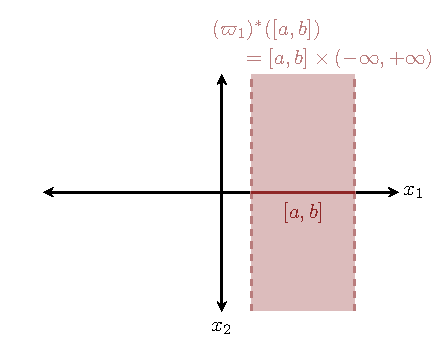
\includegraphics[width=0.5\textwidth,height=\textheight]{figures/lebesgue_pushforward/lebesgue_pushforward.pdf}

}

\caption{\label{fig-lebesgue-pushforward}On \(\mathbb{R}^{2}\), the
projection function \(\phi_{1} : (x_{1}, x_{2}) \mapsto x_{1}\) pulls
finite output space intervals \([a, b]\) back to infinite input space
rectangles \([a, b] \times (-\infty, +\infty)\). Consequently, the two
dimensional Lebesgue measure \(\lambda^{2}\) projects infinite measure
onto finite intervals, and the pushforward measure
\((\phi_{1})_{*} \lambda^{2}\) cannot be \(\sigma\)-finite. In
particular, \(\lambda^{2}\) does \emph{not} pushforward to a Lebesgue
measure on the output space!}

\end{figure}%

Fortunately, disintegrations can be generalized to work with \emph{any}
convenient \(\sigma\)-finite measure on the output space.
Mathematically, if we have

\begin{enumerate}
\def\labelenumi{\arabic{enumi}.}
\tightlist
\item
  an input measurable space \((X, \mathcal{X})\),
\item
  an input \(\sigma\)-finite, Radon measure
  \(\mu : \mathcal{X} \rightarrow [0, \infty]\),
\item
  an output Hausdorff measurable space \((Y, \mathcal{Y})\).
\item
  a surjective measurable function
  \(f: (X, \mathcal{X}) \rightarrow (Y, \mathcal{Y})\),
\item
  and finally an output \(\sigma\)-finite measure
  \(\nu : \mathcal{Y} \rightarrow [0, \infty]\),
\end{enumerate}

then there exists at least one \textbf{conditional measure kernel}
\begin{alignat*}{6}
\mu^{f, \nu} :\; &\mathcal{X} \times Y& &\rightarrow& \; &[0, \infty]&
\\
&\mathsf{x}, y& &\mapsto& &\mu^{f}( \mathsf{x} \mid y )&
\end{alignat*} that defines a
\((\mathcal{Y}, \mathcal{B}_{\mathbb{R}})\)-measurable function when
partially evaluated on any \(\mathsf{x} \in \mathcal{X}\) in the first
argument, \begin{alignat*}{6}
\mu^{f, \nu}_{\mathsf{x}} :\; &Y& &\rightarrow& \; &[0, \infty]&
\\
&y& &\mapsto& &\mu^{f, \nu}( \mathsf{x} \mid y )&,
\end{alignat*} and a \(\sigma\)-finite measure when partially evaluated
on \(\nu\)-almost any \(y \in Y\) in the second argument,
\begin{alignat*}{6}
\mu^{f}_{y, \nu} :\; &\mathcal{X}& &\rightarrow& \; &[0, \infty]&
\\
&\mathsf{x}& &\mapsto& &\mu^{f, \nu}( \mathsf{x} \mid y )&.
\end{alignat*} A more technical discussion can be found in Chang and
Pollard (1997).

The conditional measures derived from a conditional measure kernel
behave very similarly to conditional probability distributions. For
instance, they each concentrate on a particular level set, \[
\mu^{f, \nu}_{y}( f^{-1}(x) ) \overset{\nu}{=} 1
\] with \[
\mu^{f, \nu}_{y}( \mathsf{x} ) \overset{\nu}{=} 0
\] for any disjoint subset \(\mathsf{x} \cap f^{-1}(y) = \emptyset\).
Because of this concentration, if \[
\mu( \, f^{-1}(y) \, ) = 0
\] then the conditional measure \(\mu^{f, \nu}_{y}\) will \emph{not} be
absolutely continuous with respect to the initial measure!

For any well-behaved integrand \(g : X \rightarrow \mathbb{R}\), the
conditional measures also satisfy a law of total integration, \[
\int \mu( \mathrm{d} x ) \, g(x)
=
\int \nu (\mathrm{d} y)
\int \mu^{f, \nu}( \mathrm{d}x_{y} \mid y ) \,
g( \iota_{y}(x_{y})).
\]

In circumstances where \(f_{*} \mu\) happens to be \(\sigma\)-finite, we
can always take \(\nu = f_{*} \mu\) so that the law of total integration
mirrors the law of total expectation. This is always possible if \(\mu\)
is a finite measure, and hence always possible when disintegrating
probability distributions. It is not, however, always viable when
\(\mu\) is only \(\sigma\)-finite. In particular, we have to be vigilant
when attempting to disintegrate Lebesgue measures, as they often
pushforward to measures that are not \(\sigma\)-finite.

\subsection{Lebesgue Disintegrations}\label{sec:leb_disint}

In theory, the disintegration of an input space measure with respect to
an output space measure defines reference measures adapted to each level
set of a surjective function \(f: X \rightarrow Y\). This construction
isn't all that useful, however, if we cannot explicitly integrate
against these conditional reference measures. Fortunately, the
integration of conditional Lebesgue measures reduces to standard
operations from multivariate calculus.

Consider an \(N\)-dimensional space \(X = \mathbb{R}^{N}\) equipped with
a Lebesgue measure \(\mu = \lambda^{N}\) and an \(M\)-dimensional space
\(Y = \mathbb{R}^{M}\) equipped with a Lebesgue measure
\(\nu = \lambda^{M}\). Moreover, assume that \(N > M\).

In this case, any smooth, surjective function
\(f: \mathbb{R}^{N} \rightarrow \mathbb{R}^{M}\) defines level sets that
are \(\lambda^{Y}\) almost all \((N - M)\)-dimensional. These level sets
not only partition \(X\) but also disintegrate \(\mu\) into conditional
Lebesgue measures that concentrate within each of these level sets.

If \(M = N - 1\) then almost all of the level sets will be
one-dimensional. We can always completely cover the one-dimensional
level set with a countable number of one-dimensional curves through
\(X\); usually one curve is sufficient, but we have to be careful in
case, for example, the level sets are disconnected. Moreover, the
conditional integral of any function \(g : X \rightarrow \mathbb{R}\)
with respect to \(\mu^{f, \nu}\) is given but summing up the
\textbf{line integrals} Larson, Hostetler, and Edwards (1990) of \(g\)
over each of these curves.

More explicitly, let's say that the level set \(f^{-1}(y)\) can be
completely traced out by the single curve \[
\gamma_{y} : [a, b] \rightarrow X,
\] with the variable \(z \in [0, 1]\) tracking the relative position
along the curve. In this case, the conditional integral of \(g\) with
respect to \(\mu^{f, \lambda^{X}}\) can be evaluated as \begin{align*}
i_{y}
&=
\int \mu^{f, \nu}( \mathrm{d}x_{y} \mid y ) \,
g(\iota_{y}(x_{y}))
\\
&=
\int_{a}^{b} \mathrm{d} z \, J_{y}(z) \, g( \gamma_{y}(z) ),
\end{align*} where \(J_{y}(z)\) is the Jacobian correction, \[
J_{y}(z)
=
\sqrt{
  \sum_{n = 1}^{N}
  \left(
    \frac{ \mathrm{d} \gamma_{y, n} }{ \mathrm{d} z } (z)
  \right)^{2}
}.
\]

Similarly, if \(M = N - 2\) then almost level sets of any smooth,
surjective function \(f: \mathbb{R}^{N} \rightarrow \mathbb{R}^{M}\)
will be two-dimensional. These two-dimensional level sets can be covered
by a two-dimensional surfaces, with conditional measures given by
\textbf{surface integrals} over those surfaces.

To anchor all of this abstraction, let's consider an explicit example
using the two-dimensional space \(X = \mathbb{R}^{2}\) and the radial
function \begin{alignat*}{6}
f :\; &X& &\rightarrow& \; &\mathbb{R}^{+}&
\\
&(x_{1}, x_{2})& &\mapsto& &r = \sqrt{ x_{1}^{2} + x_{2}^{2} }&.
\end{alignat*}

All of the level sets of this function are concentric circles, except
for \(f^{-1}(0)\) which reduces to a singular point. Each of the
non-singular level sets can be traced out by a circular curve
(Figure~\ref{fig-rad-level-sets1}). Here we'll use the curves
\begin{alignat*}{6}
\gamma_{r} :\; &[0, 2 \, \pi )& &\rightarrow& \; &\mathbb{R}^{2}&
\\
&\theta& &\mapsto& &( r \, \cos \theta, r \, \sin \theta )&.
\end{alignat*}

\begin{figure}

\centering{


\includegraphics[width=0.5\textwidth,height=\textheight]{figures/radial_level_sets/1/1.pdf}

}

\caption{\label{fig-rad-level-sets1}The circular level sets of the
radial function
\(f: (x_{1}, x_{2}) \mapsto r = \sqrt{ x_{1}^{2} + x_{2}^{2} }\)
partition the input space \(\mathbb{R}^{2}\). All but the singular level
set \(f^{-1}(0)\) can be parameterized by one-dimensional curves, an
example of which is shown here in teal. Integrals with respect to
conditional Lebesgue measures can be evaluated as line integrals over
these curves.}

\end{figure}%

Given the Jacobian correction \begin{align*}
J_{r}
&=
\sqrt{
  \left(
    \frac{
      \mathrm{d} \gamma_{r, 1}
    }{
      \mathrm{d} \theta
    } ( \theta )
  \right)^{2}
  +
  \left(
    \frac{
      \mathrm{d} \gamma_{r, 2}
    }{
      \mathrm{d} \theta
    } ( \theta )
  \right)^{2}
}
\\
&=
\sqrt{
  \left(
    \frac{
      \mathrm{d} r \, \cos \theta
    }{
      \mathrm{d} \theta
    }
  \right)^{2}
  +
  \left(
    \frac{
      \mathrm{d} r \, \sin \theta
    }{
      \mathrm{d} \theta
    }
  \right)^{2}
}
\\
&=
\sqrt{
  \left(
    r \, \sin \theta
  \right)^{2}
  +
  \left(
    - r \, \cos \theta
  \right)^{2}
}
\\
&=
\sqrt{
  r^{2} \,
  \left(
    \sin^{2} \theta + \cos^{2} \theta
  \right)^{2}
}
\\
&=
\sqrt{
  r^{2}
}
\\
&=
r,
\end{align*} the conditional integral over one of these curves is given
by \begin{align*}
i_{r}
&=
\int \mu^{f, \nu}( \mathrm{d} x_{r} \mid r ) \,
g(\iota_{r}(x_{r}))
\\
&=
\int_{0}^{2 \, \pi} \mathrm{d} \theta \,
J_{r}(\theta) \, g( \gamma_{r}(\theta) )
\\
&=
\int_{0}^{2 \, \pi} \mathrm{d} \theta \,
r \, g( r \, \cos \theta, r \, \sin \theta ).
\end{align*}

\section{Conditional Probability Density Functions For General Implicit
Partitions}\label{conditional-probability-density-functions-for-general-implicit-partitions}

Armed with a technique for disintegrating \(\sigma\)-finite measures, we
are now finally equipped with enough tools to construct conditional
probability density functions for any conditional probability
distribution paired with a sufficiently well-behaved reference measure.

\subsection{Setup}\label{setup}

Recall that to construct a conditional probability distribution we need

\begin{enumerate}
\def\labelenumi{\arabic{enumi}.}
\tightlist
\item
  an input measurable space \((X, \mathcal{X})\),
\item
  an input Radon probability distribution
  \(\pi : \mathcal{X} \rightarrow [0, 1]\),
\item
  an output Hausdorff measurable space \((Y, \mathcal{Y})\).
\item
  and a surjective measurable function
  \(f: (X, \mathcal{X}) \rightarrow (Y, \mathcal{Y})\).
\end{enumerate}

In order to construct conditional probability density functions, we will
also need convenient \(\sigma\)-finite Radon reference measures for

\begin{enumerate}
\def\labelenumi{\arabic{enumi}.}
\setcounter{enumi}{4}
\tightlist
\item
  the input space, \(\mu : \mathcal{X} \rightarrow [0, \infty]\)
\item
  and the output space, \(\nu : \mathcal{Y} \rightarrow [0, \infty]\).
\end{enumerate}

Disintegrating the input space reference measure with respect to \(f\)
and the output space reference measure gives \(\sigma\)-finite reference
measures over each level set,

\begin{enumerate}
\def\labelenumi{\arabic{enumi}.}
\setcounter{enumi}{6}
\tightlist
\item
  \(\mu^{f, \nu} : \mathcal{F}_{y} \rightarrow [0, \infty]\).
\end{enumerate}

As we have previously discussed, we can safely take measurable
functions, Hausdorff \(\sigma\)-algebras, and Radon measures for granted
in practice. We will, however, have to be careful about the surjectivity
of \(f\) and the \(\sigma\)-finiteness of the reference measures.

If \(\pi \ll \mu\), then we can construct the probability density
function \[
\frac{ \mathrm{d}  \pi }{ \mathrm{d}  \mu  } : X \rightarrow \mathbb{R}^{+},
\] and if \(f_{*} \pi \ll \nu\) then we can construct the pushforward
probability density function \[
\frac{ \mathrm{d}  f_{*} \pi }{ \mathrm{d}  \nu  } : Y \rightarrow \mathbb{R}^{+}.
\] Upon disintegrating \(\mu\), we can construct conditional probability
density functions relative to the conditional measures, \[
\frac{ \mathrm{d}  \pi^{f} }{ \mathrm{d}  \mu^{f, \nu}  }
: X \times Y \rightarrow \mathbb{R}^{+}.
\]

\subsection{The Product Rule}\label{the-product-rule}

All that we're missing is a mathematical relationship that ties all of
these different probability density functions together. That is hidden
within the law of total expectation, \begin{align*}
\int \pi( \mathrm{d} x ) \, g(x)
&=
\int f_{*} \pi (\mathrm{d} y)
\int \pi^{f}( \mathrm{d}x_y \mid y ) \, g( \iota_{y}(x_{y}) )
\\
L
&=
R.
\end{align*} All we need to do is convert both sides of this equation
into the same kind of measure-informed integral.

Let's start with the left-hand side, \begin{align*}
L
&=
\int \pi ( \mathrm{d} x ) \, g(x)
\\
&=
\int \mu ( \mathrm{d} x ) \, \frac{ \mathrm{d} \pi}{ \mathrm{d} \mu }(x) \, g(x).
\end{align*} Disintegrating \(\mu\) with respect to \(f\) and \(\nu\)
allow us to write this as \begin{align*}
L
&=
\int \mu ( \mathrm{d} x ) \, \frac{ \mathrm{d} \pi}{ \mathrm{d} \mu }(x) \, g(x)
\\
&=
\int \nu ( \mathrm{d} y ) \,
\int \mu^{f, \nu}( \mathrm{d} x_{y} \mid y) \,
\frac{ \mathrm{d} \pi}{ \mathrm{d} \mu }( \iota_{y}(x_{y}) ) \, g( \iota_{y}(x_{y}) ).
\end{align*}

Over on the right-hand side, we have \begin{align*}
R
&=
\int f_{*} \pi (\mathrm{d} y)
\int \pi^{f}( \mathrm{d}x_{y} \mid y ) \,
g( \iota_{y}(x_{y}) )
\\
&=
\int \nu (\mathrm{d} y) \,
\frac{ \mathrm{d}  f_{*} \pi }{ \mathrm{d}  \nu  }(y) \,
\int \pi^{f}( \mathrm{d}x_{y} \mid y ) \,
g( \iota_{y}(x_{y}) )
\\
&=
\int \nu (\mathrm{d} y) \,
\frac{ \mathrm{d}  f_{*} \pi }{ \mathrm{d}  \nu  }(y) \,
\int \mu^{f, \nu} ( \mathrm{d}x_{y} \mid y ) \,
\frac{ \mathrm{d}  \pi^{f} }{ \mathrm{d}  \mu^{f, \nu}  }(x_{y} \mid y) \,
g( \iota_{y}(x_{y}) ).
\end{align*}

Because the domain of the inner measure-informed integral is single
level set, the pushforward probability density function \[
\frac{ \mathrm{d}  f_{*} \pi }{ \mathrm{d}  \nu  }(y)
\] is constant. Consequently, we can pull it inside the inner integral
to give \begin{align*}
R
&=
\int \nu (\mathrm{d} y) \,
\frac{ \mathrm{d}  f_{*} \pi }{ \mathrm{d}  \nu  }(y) \,
\int \mu^{f, \nu} ( \mathrm{d}x_{y} \mid y ) \,
\frac{ \mathrm{d}  \pi^{f} }{ \mathrm{d}  \mu^{f, \nu}  }(x_{y} \mid y) \,
g( \iota_{y}(x_{y}) )
\\
&=
\int \nu (\mathrm{d} y) \,
\int \mu^{f, \nu} ( \mathrm{d}x_{y} \mid y ) \,
\left[
  \frac{ \mathrm{d}  f_{*} \pi }{ \mathrm{d}  \nu  }(y) \,
  \frac{ \mathrm{d}  \pi^{f} }{ \mathrm{d}  \mu^{f, \nu}  }(x_{y} \mid y)
\right] \,
g( \iota_{y}(x_{y}) ).
\end{align*}

At this point, we can put these two pieces back together, \begin{align*}
&
\quad\; L = R
\\
&
\int \pi( \mathrm{d} x ) \, g(x)
\\
&\quad\quad=
\int f_{*} \pi (\mathrm{d} y)
\int \pi^{f}( \mathrm{d}x_{y} \mid y ) \, g( \iota_{y}(x_{y}) )
\\
&
\int \nu ( \mathrm{d} y ) \,
\int \mu^{f, \nu}( \mathrm{d} x_{y} \mid y) \,
\frac{ \mathrm{d} \pi}{ \mathrm{d} \mu }( \iota_{y}(x_{y}) ) \, g( \iota_{y}(x_{y}) )
\\
&\quad\quad=
\int \nu (\mathrm{d} y) \,
\int \mu^{f, \nu} ( \mathrm{d}x_{y} \mid y ) \,
\left[
  \frac{ \mathrm{d}  f_{*} \pi }{ \mathrm{d}  \nu  }(y) \,
  \frac{ \mathrm{d}  \pi^{f} }{ \mathrm{d}  \mu^{f, \nu}  }(x_{y} \mid y)
\right] \,
g( \iota_{y}(x_{y}) ).
\end{align*}

Because both sides of the equation are the same kind of measure-informed
integral, we have equality if and only if the integrands on both sides
are equal up to null subsets. In particular, we have equality for all
integrands \(g : X \rightarrow \mathbb{R}\) if and only if \[
\frac{ \mathrm{d} \pi}{ \mathrm{d} \mu }( \iota_{y}(x_{y}) )
\overset{ \nu, \mu^{f, \nu} }{ = }
\frac{ \mathrm{d}  f_{*} \pi }{ \mathrm{d}  \nu  }(y) \,
\frac{ \mathrm{d}  \pi^{f} }{ \mathrm{d}  \mu^{f, \nu}  }(x_{y} \mid y).
\]

This relationship is known as the \textbf{product rule} for probability
density functions. The product rule allows to construct the ambient
probability density function, the conditional probability density
function, or the pushforward probability density function given the
other two. For instance, if we know the ambient probability density
function and the pushforward probability density function, then the
conditional probability density function is given by \[
\frac{ \mathrm{d}  \pi^{f} }{ \mathrm{d}  \mu^{f, \nu}  } (x_{y} \mid y)
\overset{ \nu, \mu^{f, \nu} }{ = }
\frac{
  \frac{ \mathrm{d} \pi}{ \mathrm{d} \mu }( \iota_{y}(x_{y}) )
}{
  \frac{ \mathrm{d}  f_{*} \pi }{ \mathrm{d} \nu }(y)
}.
\]

Phew. Let's take a breath and summarize how far we've come!

We can condition an arbitrary probability density function \[
p(x) = \frac{ \mathrm{d} \pi}{ \mathrm{d} \mu }( x )
\] on the output point \(y \in Y\) in two steps. First, we restrict the
inputs to the points in the level set \(f^{-1}(y)\)
(Figure~\ref{fig-continuous-conditional-partitioned}\}), \[
p( \iota_{y}(x_{y}) ).
\] Next, we divide by the pushforward probability density function
evaluated at \(y\), \[
p(y) = \frac{ \mathrm{d}  f_{*} \pi }{ \mathrm{d} \nu }(y),
\] to give (Figure~\ref{fig-continuous-conditional-renormalized}), \[
p( x_{y} \mid y )
=
\frac{
  p( \iota_{y}(x_{y}) )
}{
  p(y)
}.
\]

\begin{figure}

\begin{minipage}{0.05\linewidth}
~\end{minipage}%
%
\begin{minipage}{0.45\linewidth}

\centering{

\captionsetup{labelsep=none}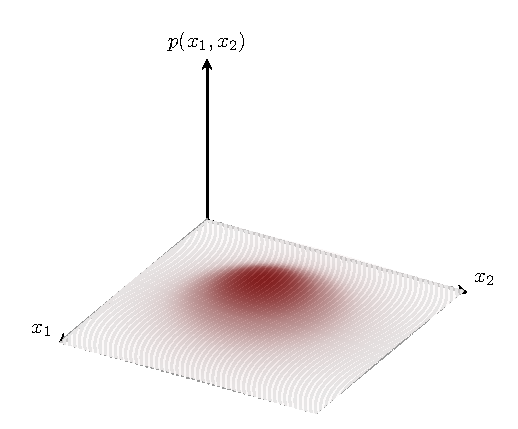
\includegraphics{figures/conditional_density_functions/continuous_partition/initial_density/initial_density.pdf}

}

\subcaption{\label{fig-continuous-conditional-initial}}

\end{minipage}%
%
\begin{minipage}{0.45\linewidth}

\centering{

\captionsetup{labelsep=none}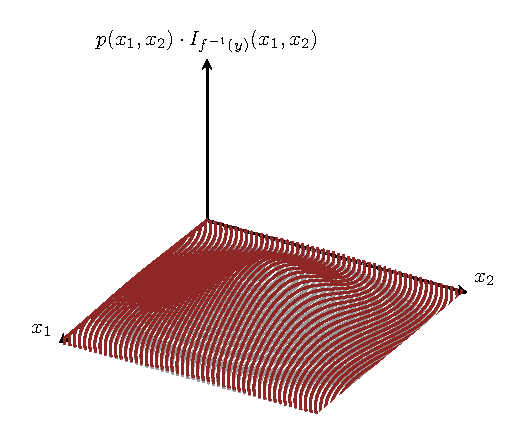
\includegraphics{figures/conditional_density_functions/continuous_partition/partitioned_densities/partitioned_densities.pdf}

}

\subcaption{\label{fig-continuous-conditional-partitioned}}

\end{minipage}%
%
\begin{minipage}{0.05\linewidth}
~\end{minipage}%
\newline
\begin{minipage}{0.28\linewidth}
~\end{minipage}%
%
\begin{minipage}{0.45\linewidth}

\centering{

\captionsetup{labelsep=none}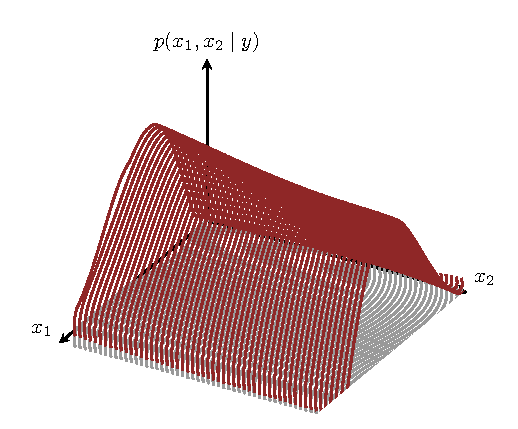
\includegraphics{figures/conditional_density_functions/continuous_partition/renormalized_densities/renormalized_densities.pdf}

}

\subcaption{\label{fig-continuous-conditional-renormalized}}

\end{minipage}%
%
\begin{minipage}{0.28\linewidth}
~\end{minipage}%

\caption{\label{fig-continuous-conditional}The product rule allows us to
generalize the construction of conditional probability density functions
that we first encountered in
\hyperref[sec:discrete-conditional-density]{Section 4.2} to any
measurable partitions. (a) An initial probability density function is
first (b) sliced into a collection of conditional density functions by
restricting valid inputs to a particular level set. (c) Dividing by the
corresponding pushforward probability density normalizes these
restricted density functions into conditional probability density
functions.}

\end{figure}%

Notice that the normalization step doesn't change the \emph{shape} of a
conditional probability density function for a given \(y\), just its
height relative to other possible values of \(y\). In applications where
we're interested in only a single \(y\), we can usually ignore this last
step, and any difficulty in evaluating the pushforward probability
density function, entirely.

\subsection{Example}\label{example}

To demonstrate this process, consider a surjective function
\(f : X \rightarrow \mathbb{N}\) that maps input points to output
integers. Because the output space is discrete, this function induces a
countable partition of the input space. Moreover, a counting measure is
a natural output reference measure, \(\nu = \chi\).

If \(f_{*} \mu( \{ y \} ) > 0\) for all \(y \in \mathbb{N}\), then each
\(\mu^{f, \chi}_{y}\) is just \(\mu\) truncated to a particular level
set, \[
\mu^{f, \chi}_{y} = \eta_{y} = I_{f^{-1}(y)} \cdot \mu.
\]

In this case, the product rule gives \begin{align*}
\frac{ \mathrm{d}  \pi^{f} }{ \mathrm{d}  \mu^{f, \chi}  } (x_{y} \mid y)
&\overset{ \mu }{ = }
\frac{
  \frac{ \mathrm{d} \pi}{ \mathrm{d} \mu }( \iota_{y}(x_{y}) )
}{
  \frac{ \mathrm{d}  f_{*} \pi }{ \mathrm{d} \chi }(y)
}
\\
&\overset{ \mu }{ = }
\frac{
  \frac{ \mathrm{d} \pi}{ \mathrm{d} \mu }( \iota_{y}(x_{y}) )
}{
  f_{*} \pi ( \{ y \} )
}
\\
&\overset{ \mu }{ = }
\frac{
  \frac{ \mathrm{d} \pi}{ \mathrm{d} \mu }( \iota_{y}(x_{y}) )
}{
  \pi ( f^{-1}(y) )
}.
\end{align*}

For a given \(y \in Y\), we can extend these conditional density
functions to all inputs \(x \in X\) by returning zero outside of the
corresponding level set, \[
\frac{ \mathrm{d}  \pi^{f} }{ \mathrm{d}  \mu^{f, \chi}  } (x \mid y)
\overset{ \mu }{ = }
\left\{
\begin{array}{rr}
\frac{ \frac{ \mathrm{d} \pi}{ \mathrm{d} \mu }(x) }{ \pi ( f^{-1}(y) ) },
& x \in f^{-1}(y)
\\
0,
& x \notin f^{-1}(y)
\end{array}
\right. ,
\] or, more compactly, \[
\frac{ \mathrm{d}  \pi^{f} }{ \mathrm{d}  \mu^{f, \chi}  } (x \mid y)
\overset{ \mu }{ = }
\frac{
  \frac{ \mathrm{d} \pi}{ \mathrm{d} \mu }(x) \, I_{f^{-1}(y)}(x)
}{
  \pi ( f^{-1}(y) )
}.
\]

This general result is consistent with the particular result that we
derived in \hyperref[sec:discrete-conditional-density]{Section 4.2}. In
other words, using the general product rule will always give us a
well-defined conditional probability density function.

\section{Explicit Formula For Pushforward Probability Density
Functions}\label{sec:push-densities}

The disintegration of reference measures is also how we can derive an
explicit formula for pushforward probability density functions.

Recall the definition of pullback expectation values: for
sufficiently-measurable functions \(f : X \rightarrow Y\) and
\(h : Y \rightarrow \mathbb{R}\), we have \begin{align*}
\mathbb{E}_{\pi} \! \left[  h \circ f  \right]
&=
\mathbb{E}_{f_{*} \pi} \! \left[  h  \right]
\\
\mathbb{I}_{\mu} \! \left[  \frac{ \mathrm{d}  \pi }{ \mathrm{d}  \mu  } \, h \circ f  \right]
&=
\mathbb{I}_{\nu} \! \left[  \frac{ \mathrm{d}  f_{*} \pi }{ \mathrm{d}  \nu  } \, h  \right],
\end{align*} or, equivalently, \begin{align*}
\int \pi( \mathrm{d} x ) \, h(f(x))
&=
\int f_{*} \pi( \mathrm{d} y )  \, h(y)
\\
\int \mu( \mathrm{d} x ) \, \frac{ \mathrm{d}  \pi }{ \mathrm{d}  \mu  }(x) \, h(f(x))
&=
\int \nu( \mathrm{d} y ) \, \frac{ \mathrm{d}  f_{*} \pi }{ \mathrm{d}  \nu  }(y) \, h(y).
\end{align*}

Disintegrating \(\mu\) with respect to \(f\) and \(\nu\) allows us to
write the left-hand side as \begin{align*}
\int \pi( \mathrm{d} x ) \, h(f(x))
&=
\int \mu( \mathrm{d} x ) \, \frac{ \mathrm{d} \pi}{ \mathrm{d} \mu }(x) \, h(f(x))
\\
&=
\int \nu( \mathrm{d} y ) \,
\int \mu^{f, \nu}( \mathrm{d} x_{y} \mid y ) \,
\frac{ \mathrm{d} \pi}{ \mathrm{d} \mu }( \iota_{y}(x_{y}) ) \, h(y).
\end{align*}

Because the function \(h \circ f : X \rightarrow \mathbb{R}\) yields the
same output for any \(x \in f^{-1}(y)\), it is a constant with respect
to the inner integral. Consequently, we can factor it out,
\begin{align*}
\int \pi( \mathrm{d} x ) \, h(f(x))
&=
\int \nu( \mathrm{d} y ) \,
\int \mu^{f, \nu}( \mathrm{d} x_{y} \mid y ) \,
\frac{ \mathrm{d} \pi}{ \mathrm{d} \mu }( \iota_{y}(x_{y}) ) \, h(y)
\\
&=
\int \nu( \mathrm{d} y )
\left[
  \int \mu^{f, \nu}( \mathrm{d} x_{y} \mid y ) \,
       \frac{ \mathrm{d} \pi}{ \mathrm{d} \mu }( \iota_{y}(x_{y}) )
\right] \, h(y).
\end{align*}

Our initial equation then becomes \begin{align*}
\int \pi( \mathrm{d} x ) \, h(f(x))
&=
\int f_{*} \pi( \mathrm{d} y ) \, h(y)
\\
\int \nu( \mathrm{d} y )
\left[
  \int \mu^{f, \nu}( \mathrm{d} x_{y} \mid y ) \,
       \frac{ \mathrm{d} \pi}{ \mathrm{d} \mu }( \iota_{y}(x_{y}) )
\right] \, h(y)
&=
\int \nu( \mathrm{d} y ) \,
\left[ \frac{ \mathrm{d} f_{*}\pi}{ \mathrm{d} \nu }(y) \right] \, h(y).
\end{align*}

Because both sides of this equation are \(\nu\)-informed integrals, we
have equality if and only if the integrands are equal up to \(\nu\)-null
subsets. In particular, we have equality for any integrand
\(h : Y \rightarrow \mathbb{R}\) if and only if \[
\frac{ \mathrm{d} f_{*}\pi}{ \mathrm{d} \nu }(y)
\overset{\nu}{=}
\int \mu^{f, \nu}( \mathrm{d} x_{y} \mid y ) \,
\frac{ \mathrm{d} \pi}{ \mathrm{d} \mu }( \iota_{y}(x_{y}) ).
\]

In theory, this gives us an explicit formula for deriving pushforward
probability density functions. Implementing this result in practice,
however, requires an explicit method for evaluating conditional
integrals over each level set of \(f\). Fortunately, we know how to do
this when working with real spaces and Lebesgue measures.

Consider, for example, the two-dimensional positive real space
\(X = \mathbb{R}^{+} \times \mathbb{R}^{+}\) equipped with a Lebesgue
measure \(\mu = \lambda^{2}\), a Lebesgue probability density function
\[
p(x_{1}, x_{2}) = \frac{ \mathrm{d} \pi}{ \mathrm{d} \mu }(x_{1}, x_{2}),
\] and the radial function \begin{alignat*}{6}
f :\; &X& &\rightarrow& \; &\mathbb{R}^{+}&
\\
&(x_{1}, x_{2})& &\mapsto& &r = \sqrt{ x_{1}^{2} + x_{2}^{2} }&.
\end{alignat*}

Because \(X\) is restricted to non-negative values, the level sets of
\(f\) define not entire circles but rather circular arcs
(Figure~\ref{fig-rad-level-sets2}). We'll cover these arcs with the
curves \begin{alignat*}{6}
\gamma_{r} :\; &[0, \pi / 2 )& &\rightarrow& \; &X&
\\
&\theta& &\mapsto& &( r \, \cos \theta, r \, \sin \theta )&.
\end{alignat*}

\begin{figure}

\centering{


\includegraphics[width=0.5\textwidth,height=\textheight]{figures/radial_level_sets/2/2.pdf}

}

\caption{\label{fig-rad-level-sets2}When the inputs are restricted to
non-negative values, the level sets of the radial function
\(f: (x_{1}, x_{2}) \mapsto r = \sqrt{ x_{1}^{2} + x_{2}^{2} }\)
partition the input space into circular arcs, each of which can be
parameterized with a curve of constant radius, one of which an is shown
here in teal. Integrals with respect to conditional Lebesgue measures
can be evaluated as line integrals over these curves.}

\end{figure}%

In this case, the Jacobian correction is the same as it was for the
example of \hyperref[sec:leb_disint]{Section 4.2}, \[
J_{r} = r.
\] Consequently, we write the pushforward probability density function
as (Figure~\ref{fig-radial1-pushforward}) \begin{align*}
p(r)
&=
\int_{0}^{ \frac{\pi}{2} } \mathrm{d} \theta \,
J_{r}(\theta) \, p( \gamma_{r}(\theta) )
\\
&=
\int_{0}^{ \frac{\pi}{2} } \mathrm{d} \theta \,
r \, p( r \, \cos \theta, r \, \sin \theta ).
\end{align*} At this point, we can use the product rule to construct the
conditional probability density function over each level set
(Figure~\ref{fig-radial1-conditional}), \[
p(\theta_{r} \mid r) = \frac{ p(r, \theta_{r}) }{ p(r) }.
\]

\begin{figure}

\begin{minipage}{0.05\linewidth}
~\end{minipage}%
%
\begin{minipage}{0.45\linewidth}

\centering{

\captionsetup{labelsep=none}
\includegraphics{figures/radial1/initial/initial.pdf}

}

\subcaption{\label{fig-radial1-initial}}

\end{minipage}%
%
\begin{minipage}{0.45\linewidth}

\centering{

\captionsetup{labelsep=none}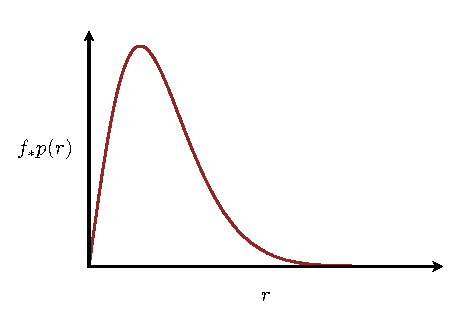
\includegraphics{figures/radial1/pushforward/pushforward.pdf}

}

\subcaption{\label{fig-radial1-pushforward}}

\end{minipage}%
%
\begin{minipage}{0.05\linewidth}
~\end{minipage}%
\newline
\begin{minipage}{0.28\linewidth}
~\end{minipage}%
%
\begin{minipage}{0.45\linewidth}

\centering{

\captionsetup{labelsep=none}
\includegraphics{figures/radial1/conditional/conditional.pdf}

}

\subcaption{\label{fig-radial1-conditional}}

\end{minipage}%
%
\begin{minipage}{0.28\linewidth}
~\end{minipage}%

\caption{\label{fig-radial1}When we have the computational tools to
evaluate conditional integrals over level sets, we can evaluate
pushforward probability density functions. Here we integrate (a) an
initial density function over circular level sets to derive (b) a
pushforward probability density function over output radii. (c)
Restricting the initial probability density function to a level set and
then dividing by corresponding pushforward probability density gives the
conditional probability density function for that level set.}

\end{figure}%

Even when we can reduce conditional integrals to line integrals,
however, evaluating the resulting line integrals in closed form can be a
challenge. For those with a taste for tricky integrals, I work through
an explicit example that requires some uncommon mathematical functions
in the \hyperref[sec:appendix]{Appendix}.

\section{Conditional Building Blocks}\label{conditional-building-blocks}

To this point, we have discussed conditional probability theory as a
tool for \emph{breaking} probability distributions down into simpler
pieces. Conditional probability theory, however, can also be used to
\emph{build} probability distributions up from simpler pieces.
Throughout this section, I will take the technical requirements of Radon
measures and Hausdorff \(\sigma\)-algebras for granted.

\subsection{One Step}\label{one-step}

Given a probability distribution \(\pi\) defined over the space \(X\), a
measurable, surjective function \(f : X \rightarrow Y\) defines both a
pushforward probability distribution \(f_{*} \pi\) over the output space
of \(f\) and a conditional probability kernel \(\pi^{f}\) over the level
sets of \(f\). Through the laws of total probability and total
expectation, we can always reconstruct any probabilistic operation with
respect to \(\pi\) from these two byproducts alone.

This construction also works the other way around. Given a measurable,
surjective function \(f: X \rightarrow Y\), any probability distribution
over the output space, \(\rho\), and conditional probability kernel over
the level sets, \begin{alignat*}{6}
\tau :\; &\mathcal{X} \times Y& &\rightarrow& \; &[0, 1]&
\\
&\mathsf{x}, y& &\mapsto& &\tau ( \mathsf{x} \mid y )&,
\end{alignat*} uniquely defines a probability distribution \(\pi\) over
\(X\) through the law of total probability, \[
\pi( \mathsf{x} ) = \mathbb{E}_{\rho} [ t_{\mathsf{x}} ],
\] where \begin{alignat*}{6}
t_{\mathsf{x}} :\; &Y& &\rightarrow& \; &[0, 1]&
\\
&y& &\mapsto& &\tau ( \mathsf{x} \mid y )&.
\end{alignat*} In this case, we say that \(\tau\) \textbf{lifts}
\(\rho\) into a probability distribution over \(X\).

Lifting allows us to construct probability distributions over \(X\) in
steps, first specifying the probabilistic structure over \(Y\) and then
filling in any missing information with conditional probabilistic
strucure across the levels sets. If \(Y\) is a much simpler space than
\(X\), for example a lower-dimensional space with fewer degrees of
freedom to consider, and the level sets of \(f\) are straightforward to
interpret, then this sequential procedure can be much easier to
implement in practice than trying to define a probability distribution
over \(X\) all at once.

Equivalently, we can define a lifted probability distribution through
its expectation values with the law of total expectation, \[
\int \pi( \mathrm{d} x ) \, g(x)
=
\int \rho (\mathrm{d} y)
\int \tau( \mathrm{d}x_{y} \mid y ) \, g(x).
\] The advantage of this latter approach is that it allows us to
implicitly define \(\pi\) through a sequence of probability density
functions.

Given an output reference measure \(\nu\), any sufficiently well-behaved
function \[
r : Y \rightarrow \mathbb{R}^{+}
\] with \(\mathbb{I}_{\nu}[ r ] = 1\) defines an output probability
distribution \(\rho = r \, \nu\) through the expectation values \[
\int \rho( \mathrm{d} y ) h(y)
=
\int \nu (\mathrm{d} y) \, r(y) \, h(y).
\] Similarly, given an input reference measure \(\mu\) and its
disintegration \(\mu^{f, \nu}\), any sufficiently well-behaved binary
function \[
t : X \times Y \rightarrow \mathbb{R}^{+}
\] with \[
\mathbb{I}_{\mu^{f, \nu}_{y}}[ t ] \overset{\nu}{=} 1
\] defines a conditional probability kernel \(\tau = t \, \mu^{f, \nu}\)
through the conditional expectation values \[
\int \tau( \mathrm{d} x_{y} \mid y) \,
g( \iota_{y}(x_{y}) )
=
\int \mu^{f, \nu}( \mathrm{d} x_{y} \mid y) \,
\tau(x_{y} \mid y) \, g( \iota_{y}(x_{y}) ).
\]

By construction, the product of these two functions, \[
p( \iota_{y}(x_{y}) ) = t(x_{y} \mid y ) \, r( y ),
\] will always satisfy \begin{align*}
\mathbb{I}_{\mu} [ p ]
&=
\int \mu( \mathrm{d} x) p(x)
\\
&=
\int \nu( \mathrm{d} y)
\int \mu^{f, \nu}( \mathrm{d}x_{y} \mid y ) \,
p( \iota_{y}(x_{y}) )
\\
&=
\int \nu( \mathrm{d} y)
\int \mu^{f, \nu}( \mathrm{d}x_{y} \mid y ) \,
t(x_{y} \mid y ) \, r( y )
\\
&=
\int \nu( \mathrm{d} y) \, r( y ) \,
\int \mu^{f, \nu}( \mathrm{d}x_{y} \mid y ) \, t(x_{y} \mid y )
\\
&=
\int \nu( \mathrm{d} y) \, r( y )
\\
&=
1.
\end{align*} Consequently, \(\pi = p \, \mu\) defines a probability
distribution over the input space with the expectation values
\begin{align*}
\int \pi( \mathrm{d}x ) \, g(x)
&=
\int \rho (\mathrm{d}y)
\int \tau( \mathrm{d}x_{y} \mid y ) \, g( \iota_{y}(x_{y}) )
\\
&=
\int \nu (\mathrm{d}x ) \, r(y) \,
\int \mu^{f, \nu}( \mathrm{d}x_{y} \mid y) \,
t(x_{y} \mid y) \, g( \iota_{y}(x_{y}) ).
\end{align*}

\subsection{Of Many}\label{of-many}

While simpler than an ambient probability distribution, an output
probability distribution can still be too overwhelming to construct
directly. Fortunately, we can always apply this sequential construction
again, building up the initial output probability distribution from a
new conditional probability kernel, and a new, even simpler output
probability distribution. In turn, that new output probability
distribution can be built up from simpler pieces, and so on.

More formally, consider a sequence of \(N + 1\) spaces, \[
\{ X_{0}, \ldots, X_{n}, \ldots, X_{N} \},
\] that become increasingly more manageable. For example, the dimension
of each space might decrease as the sequence progresses.

Given surjective functions that relate each pair of neighboring spaces,
\begin{align*}
f_{1} :& \, X_{0} \rightarrow X_{1}
\\
&\ldots
\\
f_{n} :& \, X_{n - 1} \rightarrow X_{n}
\\
&\ldots
\\
f_{N} :& \, X_{N - 1} \rightarrow X_{N},
\end{align*} we can building up a probability distribution over
\(X_{0}\) from a terminal probability distribution \(\pi_{N}\) over
\(X_{N}\) and a sequence of conditional probability kernels defined over
the level sets of each \(f_{n}\), \[
\{ \tau_{N}, \ldots, \tau_{n}, \ldots, \tau_{1} \}.
\] In other words, we can \emph{incrementally} build up sophisticated
probability distributions over \(X_{0}\) from a sequence of simpler,
more manageable pieces.

When all of the spaces \(X_{n}\) are equipped with well-behaved
reference measures, we can specify the probability distribution over
\(X_{0}\) with a probability density function built up from the product
of a terminal probability density function, \[
p_{N} : X_{N} \rightarrow \mathbb{R}^{+},
\] and a sequence of conditional probability density functions, \[
t_{n} : X_{n - 1} \times X_{n} \rightarrow \mathbb{R}^{+}.
\]

For example, applying the product rule once gives a probability density
function over \(X_{N - 1}\), \[
p_{N - 1}( x_{N - 1} ) =
t_{N}( x_{N - 1} \mid x_{N} ) \,
p_{N} ( x_{N} ),
\] where \(x_{N}\) is implicitly defined by \[
x_{N} = f_{N}( x_{N - 1} ).
\] Applying it twice defines a probability density function over
\(X_{N - 2}\), \begin{align*}
p_{N - 2}( x_{N - 2} )
&=
t_{N - 1}( x_{N - 2} \mid x_{N - 1} ) \,
p_{N - 1} ( x_{N - 1} )
\\
&=
t_{N - 1}( x_{N - 2} \mid x_{N - 1} ) \,
t_{N}( x_{N - 1} \mid x_{N} ) \,
p_{N} (x_{N} ),
\end{align*} where \begin{align*}
x_{N - 1} &= f_{N - 1}( x_{N - 2} )
\\
x_{N}     &= f_{N}( x_{N - 1} ).
\end{align*}

Repeatedly applying the product rule \(N - 2\) more times gives a
probability density function over \(X_{0}\), \[
p_{0}( x_{0} )
=
\left[
  \prod_{n = 1}^{N} t_{n}( x_{n - 1} \mid x_{n} )
\right] \,
p_{N} (x_{N}),
\] where the variables \[
\{ x_{1}, \ldots, x_{N} \}
\] are completely determined by \(x_{0}\) through the recursive
constraints \[
x_{n} = f_{n}( x_{n - 1} ).
\]

\subsection{Example}\label{sec:build-ex}

To demonstrate the sequential construction of a probability density
function, let's consider the input space
\(X = \mathbb{R} \times \mathbb{R}\) equipped with a Lebesgue measure
and our now familiar radial function, \begin{alignat*}{6}
f :\; &X& &\rightarrow& \; &\mathbb{R}^{+}&
\\
&(x_{1}, x_{2})& &\mapsto& &r = \sqrt{ x_{1}^{2} + x_{2}^{2} }&.
\end{alignat*}

Assuming the local Lebesgue measure over \(Y = \mathbb{R}^{+}\), we can
construct an output probability distribution with a probability density
function of the form \[
p(r) =
\frac{ \beta^{\alpha} }{ \Gamma( \alpha ) }
r^{\alpha - 1} \exp( - \beta \, r )
\] for any \(\alpha, \beta \in \mathbb{R}^{+}\). Here \(\Gamma(x)\) is
the Gamma function (Abramowitz and Stegun 1964).

After disintegrating the input Lebesgue measure over \(X\) with respect
to \(f\) and an output Lebesgue measure over \(Y\), we can define define
conditional probability distributions over each level set of \(f\) with
the conditional probability density functions \[
p( \theta_{r} \mid r )
=
\frac{1}{2 \, \pi \, I_{0}(\kappa) }
\exp( \, \kappa \, \cos( \theta_{r} - \pi \, r) \, ).
\] Here \(I_{0}(x)\) is the modified Bessel function of the first kind
(Abramowitz and Stegun 1964).

Together, these two pieces immediately define a probability density
function over \(X\), \[
p( x_{1}, x_{2} )
=
p( \theta_{r} \mid r ) \, p( r ),
\] where \(r\) and \(\theta_{r}\) are completely determined by \(x_{1}\)
and \(x_{2}\). To make this easier to apply in practice, we'll need to
work out this dependence explicitly.

The radial function gives an equation for the radius in terms of
\(x_{1}\) and \(x_{2}\), \[
r = f(x_{1}, x_{2}) = \sqrt{ x_{1}^{2} + x_{2}^{2} },
\] but the angular position along the corresponding level set is a bit
more subtle.

Recall that the inclusion map defines \begin{align*}
x_{1} &= r \, \cos \theta_{r}
\\
x_{2} &= r \, \sin \theta_{r}.
\end{align*} If \(x_{1}\) is positive, then we can divide the two
equations to give \[
\frac{ x_{2} }{ x_{1} }
=
\tan \theta_{r}
\] or \[
\theta_{r} = \arctan \left( \frac{ x_{2} }{ x_{1} } \right).
\] More generally, the angular position is given by the output of the
two-argument inverse tangent function, \[
\theta_{r}
=
\mathrm{atan2}(x_{2}, x_{1})
=
\left\{
\begin{array}{ll}
\arctan(x_{2} / x_{1}),       & x_{1} > 0           \\
\arctan(x_{2} / x_{1}) + \pi, & x_{1} < 0, x_{2} \ge 0, \\
\arctan(x_{2} / x_{1}) - \pi, & x_{1} < 0, x_{2} < 0,   \\
+ \pi / 2,                    & x_{1} = 0, x_{2} > 0,   \\
- \pi / 2,                    & x_{1} = 0, x_{2} < 0,   \\
\mathrm{undefined},           & x_{1} = 0, x_{2} = 0
\end{array}
\right. .
\]

With the radial and two-argument inverse tangent functions, we can write
the ambient probability density function as (Figure~\ref{fig-radial2}),
\[
p( x_{1}, x_{2} )
=
p( \mathrm{atan2}(x_{2}, x_{1}) \mid
   \sqrt{ x_{1}^{2} + x_{2}^{2} } ) \,
p( \sqrt{ x_{1}^{2} + x_{2}^{2} } ).
\]

\begin{figure}

\begin{minipage}{0.05\linewidth}
~\end{minipage}%
%
\begin{minipage}{0.45\linewidth}

\centering{

\captionsetup{labelsep=none}
\includegraphics{figures/radial2/marginal/marginal.pdf}

}

\subcaption{\label{fig-radial2-marginal}}

\end{minipage}%
%
\begin{minipage}{0.45\linewidth}

\centering{

\captionsetup{labelsep=none}
\includegraphics{figures/radial2/conditional/conditional.pdf}

}

\subcaption{\label{fig-radial2-pushforward}}

\end{minipage}%
%
\begin{minipage}{0.05\linewidth}
~\end{minipage}%
\newline
\begin{minipage}{0.28\linewidth}
~\end{minipage}%
%
\begin{minipage}{0.45\linewidth}

\centering{

\captionsetup{labelsep=none}
\includegraphics{figures/radial2/full/full.pdf}

}

\subcaption{\label{fig-radial2-conditional}}

\end{minipage}%
%
\begin{minipage}{0.28\linewidth}
~\end{minipage}%

\caption{\label{fig-radial2}Conditional probability theory can be used
to construct sophisticated probability density functions from simpler
pieces. Given a function \(f: X \rightarrow Y\) and appropriate
reference measures, any (a) output probability density function over
\(Y\) and (b) conditional probability density functions over the level
sets \(f^{-1}(y)\) define (c) a probability density function over
\(X\).}

\end{figure}%

\section{Conditional Independence}\label{conditional-independence}

In
\href{http://www.symplectomorphic.com/assets/chapters_html/conditional_probability_theory.html\#sec:independence}{Chapter
8, Section 4}, we discussed various notions of conditional independence.
The most relevant being when the conditional probability distributions
in a conditional probability kernel behave the same across almost all
level sets.

Conditional independence imposes strong structural constraints on
conditional probability density functions. In particular, any
conditional probability density functions defined relative to the
disintegration of an ambient reference measure must be the same for all
values of the output variable \(y\). In this case, the product rule
becomes \[
\frac{ \mathrm{d}  \pi }{ \mathrm{d}  \mu  } (y, x_{y})
\overset{\mu}{=}
\frac{ \mathrm{d}  \pi^{f} }{ \mathrm{d}  \mu^{f, \nu}  } (x_{y}) \,
\frac{ \mathrm{d}  f_{*} \pi }{ \mathrm{d}  \nu  } (y),
\] or, using less explicit but more compact notation, \[
p(x) = p( x_{y} ) \, p(y).
\] Regardless of which level set \(f^{-1}(y)\) we choose, the
conditional behavior is the same.

This result suggests a straightforward procedure for constructing
probability distributions that are conditional independent with respect
to a function \(f : X \rightarrow Y\). Any function
\(p : Y \rightarrow \mathbb{R}^{+}\) with
\(\mathbb{I}_{\nu} \! \left[ r \right] = 1\) implicitly defines an
output probability distribution over \(Y\). If the level sets
\(f^{-1}(y)\) are almost all equivalent to some common space \(L\), then
any function \(l : L \rightarrow \mathbb{R}^{+}\) with
\(\mathbb{I}_{\mu^{f, \nu}} \! \left[ l \right] = 1\) implicitly defines
a probability distribution over the common level set space. The product
of these two functions, \[
p(x) = l( x_{f(x)} ) \cdot p( f(x) ),
\] defines a probability distribution over \(X\) that is conditionally
independent of \(f\).

Consider, for instance, the example from \hyperref[sec:build-ex]{Section
6.3} only with conditional probability density functions that are
independent of \(r\), \begin{align*}
p( \theta_{r} \mid r )
&=
\frac{1}{2 \, \pi \, I_{0}(\kappa) }
\exp( \, \kappa \, \cos( \theta_{r} - \pi / 3) \, )
\\
&\equiv
p( \theta_{r} ).
\end{align*}

The resulting probability density function still varies with radius and
angle, but the dependencies are independent of each other
(Figure~\ref{fig-radial3}), \[
p( x_{1}, x_{2} )
=
p( \mathrm{atan2}(x_{2}, x_{1}) ) \,
p( f(x_{1}, x_{2}) ).
\]

\begin{figure}

\begin{minipage}{0.05\linewidth}
~\end{minipage}%
%
\begin{minipage}{0.45\linewidth}

\centering{

\captionsetup{labelsep=none}
\includegraphics{figures/radial3/marginal/marginal.pdf}

}

\subcaption{\label{fig-radial3-marginal}}

\end{minipage}%
%
\begin{minipage}{0.45\linewidth}

\centering{

\captionsetup{labelsep=none}
\includegraphics{figures/radial3/conditional/conditional.pdf}

}

\subcaption{\label{fig-radial3-pushforward}}

\end{minipage}%
%
\begin{minipage}{0.05\linewidth}
~\end{minipage}%
\newline
\begin{minipage}{0.28\linewidth}
~\end{minipage}%
%
\begin{minipage}{0.45\linewidth}

\centering{

\captionsetup{labelsep=none}
\includegraphics{figures/radial3/full/full.pdf}

}

\subcaption{\label{fig-radial3-conditional}}

\end{minipage}%
%
\begin{minipage}{0.28\linewidth}
~\end{minipage}%

\caption{\label{fig-radial3}(b) By using the same conditional
probability density function for almost all level sets \(f^{-1}(y)\),
(c) the derived probability distribution over \(X\) is conditionally
independent of the function \(f\). The only radial dependence comes from
(a) the output probability distribution.}

\end{figure}%

\section{Conclusion}\label{conclusion}

Ultimately, the properties of conditional probability density functions
are relatively straightforward, despite the technical minefield we had
to navigate to derive them.

Provided that we use consistent reference measures, we can condition an
initial probability density function with respect to a function by
computing the pushforward probability density function and dividing. At
the same time, multiplying an output probability density function and a
conditional density function defines a probability density function over
the ambient space.

Aside from the general difficulty of conditional integration, the main
frustration with conditional probability density functions is one of
notation. If we make the conditioning function and its level sets
explicit, then the equations can become dense and awkward to parse. On
the other hand, if we hide these details, then the equations can be
prone to misinterpretation.

Fortunately, much of this frustration is ameliorated when we apply
conditional probability theory to \emph{product spaces} and their
natural projection functions. We'll explore this application in detail
in the \textbf{next chapter}.

\section*{Appendix: ``Explicit'' Calculations}\label{sec:appendix}
\addcontentsline{toc}{section}{Appendix: ``Explicit'' Calculations}

In this appendix, I've sequestered the nasty integrals that arise when
deriving the pushforward probability density function, and the
subsequent conditional probability density functions, shown in
Figure~\ref{fig-radial1}. This section is completely optional!

We begin with a two-dimensional, non-negative real space
\(X = \mathbb{R}^{+} \times \mathbb{R}^{+}\), equipped with a Lebesgue
reference measure and the Lebesgue probability density function
\begin{align*}
p(x_{1}, x_{2})
&=
\frac{
\exp \left( - \frac{1}{2 \, s^{2}} \frac{1}{1 - \rho^{2}}
              ( x^{2} - 2 \, \rho \, x \, y + y^{2} ) \right)
}{
\int_{0}^{\infty} \int_{0}^{\infty}
\mathrm{d} x_{1} \, \mathrm{d} x_{2} \,
\exp \left( - \frac{1}{2 \, s^{2}} \frac{1}{1 - \rho^{2}}
             ( x^{2} - 2 \, \rho \, x \, y + y^{2} ) \right).
}
\\
&=
C \,
\exp \left(
  - \frac{1}{2 \, s^{2}} \frac{1}{1 - \rho^{2}}
    ( x^{2} - 2 \, \rho \, x \, y + y^{2} )
\right),
\end{align*}

Our goal will be to condition this probability density function with
respect to the surjective radial function \begin{alignat*}{6}
f :\; &X& &\rightarrow& \; &\mathbb{R}^{+}&
\\
&(x_{1}, x_{2})& &\mapsto& &r = \sqrt{ x_{1}^{2} + x_{2}^{2} }&.
\end{alignat*}

The level sets of \(f\) are given by angular arcs of constant radius
which we can cover with the curves \begin{alignat*}{6}
\gamma_{r} :\; &[0, \pi / 2 )& &\rightarrow& \; &X&
\\
&\theta& &\mapsto& &( r \, \cos \theta, r \, \sin \theta )&.
\end{alignat*}

As we saw in \hyperref[sec:push-densities]{Section 6}, evaluating the
pushforward probability density function at any output \(r\) requires
computing the line integral \begin{align*}
p(r)
&=
\int_{0}^{ \frac{\pi}{2} } \mathrm{d} \theta \,
J_{r}(\theta) \, p( \gamma_{r}(\theta) )
\\
&=
\int_{0}^{ \frac{\pi}{2} } \mathrm{d} \theta \,
r \, p( r \, \cos \theta, r \, \sin \theta ).
\end{align*}

Now the initial probability density function written in terms of the
output radius and level set angular position simplifies to
\begin{align*}
p( r \, &\cos \theta, r \, \sin \theta )
\\
&=
C \, \exp \left(
  - \frac{1}{2 \, s^{2}} \frac{1}{1 - \rho^{2}}
    (
        (r \, \cos \theta)^{2}
      - 2 \, \rho \, r \, \cos \theta \, r \, \sin \theta
      + (r \, \sin \theta)^{2}
    )
\right)
\\
&=
C \, \exp \left(
  - \frac{1}{2 \, s^{2}} \frac{1}{1 - \rho^{2}}
(   r^{2} \, \cos^{2} \theta
  - 2 \, \rho \, r^{2} \, \cos \theta \, \sin \theta
  + r^{2} \, \sin^{2} \theta )
\right)
\\
&=
C \, \exp \left(
  - \frac{1}{2 \, s^{2}} \frac{r^{2}}{1 - \rho^{2}}
(   \sin^{2} \theta
  + \cos^{2} \theta
  - 2 \, \rho \, \sin \theta \, \cos \theta )
\right)
\\
&=
C \, \exp \left(
  - \frac{1}{2 \, s^{2}} \frac{r^{2}}{1 - \rho^{2}}
    ( 1 - 2 \, \rho \, \sin \theta \, \cos \theta )
\right)
\\
&=
C \, \exp \left(
  - \frac{1}{2 \, s^{2}} \frac{r^{2}}{1 - \rho^{2}}
  ( 1 - \rho \, \sin 2 \theta)
\right).
\end{align*}

Consequently, \begin{align*}
p(r)
&=
\int_{0}^{\frac{\pi}{2}} \mathrm{d} \theta \, r \,
p( r \, \cos \theta, r \, \sin \theta )
\\
&=
\int_{0}^{\frac{\pi}{2}} \mathrm{d} \theta \,
C \, r \, \exp \left( - \frac{1}{2 \, s^{2}} \frac{r^{2}}{1 - \rho^{2}}
( 1 - \rho \, \sin 2 \theta)
\right)
\\
&=
C \, r \,
\int_{0}^{\frac{\pi}{2}} \mathrm{d} \theta \,
\exp \left( - \frac{1}{2 \, s^{2}} \frac{r^{2}}{1 - \rho^{2}}
\right) \,
\exp \left( + \frac{1}{2 \, s^{2}} \frac{r^{2}}{1 - \rho^{2}} \,
              \rho \, \sin 2 \theta
\right)
\\
&=
C \, r \,
\exp \left(
  - \frac{1}{2 \, s^{2}} \frac{r^{2}}{1 - \rho^{2}}
\right) \,
\int_{0}^{\frac{\pi}{2}} \mathrm{d} \theta \,
\exp \left(
  + \frac{r^{2}}{2 \, s^{2}} \frac{\rho}{1 - \rho^{2}} \,
    \sin 2 \theta
\right)
\\
&\equiv
C \, r \,
\exp \left(
  - \frac{1}{2 \, s^{2}} \frac{r^{2}}{1 - \rho^{2}}
\right) \,
i(r, \rho, \theta).
\end{align*}

Conveniently, this integral can be reduced to special functions, albeit
not necessarily common ones, \begin{align*}
i(r, \rho, \theta)
&=
\int_{0}^{\frac{\pi}{2}} \mathrm{d} \theta \,
\exp \left(
  + \frac{r^{2}}{2 \, s^{2}} \frac{\rho}{1 - \rho^{2}} \,
    \sin 2 \theta
\right)
\\
&=
\frac{1}{2} \int_{0}^{\pi} \mathrm{d} \phi \,
\exp \left(
  + \frac{r^{2}}{2 \, s^{2}} \frac{\rho}{1 - \rho^{2}} \,
    \sin \phi
\right)
\\
&=
\frac{\pi}{2} \left(
  I_{0} \left(
    \frac{r^{2}}{2 \, s^{2}} \frac{\rho}{1 - \rho^{2}}
  \right)
+ L_{0} \left(
    \frac{r^{2}}{2 \, s^{2}} \frac{\rho}{1 - \rho^{2}}
  \right)
\right),
\end{align*} where \(I_{0}(x)\) is the \textbf{zeroth-order modified
Bessel function of the first kind} and \(L_{0}(x)\) is the
\textbf{zeroth-order modified Struve function} (Abramowitz and Stegun
1964).

Using this result, the pushforward probability density function becomes
\begin{align*}
p(r)
&=
C \, r \,
\exp \left(
  - \frac{1}{2 \, s^{2}} \frac{r^{2}}{1 - \rho^{2}}
\right) \,
\iota(r, \rho, \theta)
\\
&=
\frac{\pi}{2} \, C \, r \,
\exp \left(
  - \frac{1}{2 \, s^{2}} \frac{r^{2}}{1 - \rho^{2}}
\right) \,
\left(
  I_{0} \left(
    \frac{r^{2}}{2 \, s^{2}} \frac{\rho}{1 - \rho^{2}}
  \right)
+ L_{0} \left(
    \frac{r^{2}}{2 \, s^{2}} \frac{\rho}{1 - \rho^{2}}
  \right)
\right).
\end{align*}

Once we have calculated the pushfoward probability density function in
closed form, the conditional probability density function immediately
follows, \begin{align*}
p(\theta \mid r)
&=
\frac{ p(r, \theta) }{ p(r) }
\\
&=
\frac{
C \, r \, \exp \left(
  - \frac{1}{2 \, s^{2}} \frac{r^{2}}{1 - \rho^{2}}
    ( 1 - \rho \, \sin 2 \theta)
\right)
}{
\frac{\pi}{2} \, C \, r \,
\exp \left(
  - \frac{1}{2 \, s^{2}} \frac{r^{2}}{1 - \rho^{2}}
\right) \,
\left(
  I_{0} \left(
    \frac{r^{2}}{2 \, s^{2}} \frac{\rho}{1 - \rho^{2}}
  \right)
+ L_{0} \left(
    \frac{r^{2}}{2 \, s^{2}} \frac{\rho}{1 - \rho^{2}}
  \right)
\right)
}
\\
&=
\frac{
\exp \left(
  - \frac{1}{2 \, s^{2}} \frac{r^{2}}{1 - \rho^{2}}
    ( 1 - \rho \, \sin 2 \theta)
\right)
}{
\frac{\pi}{2} \,
\exp \left(
  - \frac{1}{2 \, s^{2}} \frac{r^{2}}{1 - \rho^{2}}
\right) \,
\left(
  I_{0} \left(
    \frac{r^{2}}{2 \, s^{2}} \frac{\rho}{1 - \rho^{2}}
  \right)
+ L_{0} \left(
    \frac{r^{2}}{2 \, s^{2}} \frac{\rho}{1 - \rho^{2}}
  \right)
\right)
}
\\
&=
\frac{2}{\pi} \,
\frac{
\exp \left(
  - \frac{1}{2 \, s^{2}} \frac{r^{2}}{1 - \rho^{2}}
    ( 1 - \rho \, \sin 2 \theta)
  + \frac{1}{2 \, s^{2}} \frac{r^{2}}{1 - \rho^{2}}
\right)
}{
  I_{0} \left(
    \frac{r^{2}}{2 \, s^{2}} \frac{\rho}{1 - \rho^{2}}
  \right)
+ L_{0} \left(
    \frac{r^{2}}{2 \, s^{2}} \frac{\rho}{1 - \rho^{2}}
  \right)
}
\\
&=
\frac{2}{\pi} \,
\frac{
\exp \left(
  - \frac{1}{2 \, s^{2}} \frac{r^{2}}{1 - \rho^{2}}
    (- \rho \, \sin 2 \theta)
\right)
}{
  I_{0} \left(
    \frac{r^{2}}{2 \, s^{2}} \frac{\rho}{1 - \rho^{2}}
  \right)
+ L_{0} \left(
    \frac{r^{2}}{2 \, s^{2}} \frac{\rho}{1 - \rho^{2}}
  \right)
}
\\
&=
\frac{2}{\pi} \,
\frac{
\exp \left(+ \alpha(r) \, \sin 2 \theta \right)
}{
  I_{0} \left( \alpha(r) \right) + L_{0} \left( \alpha(r) \right)
},
\end{align*} where \[
\alpha(r) = \frac{r^{2}}{2 \, s^{2}} \frac{\rho}{1 - \rho^{2}}.
\]

By construction, each individual conditional probability density
function is guaranteed to be properly normalized, \begin{align*}
\int_{0}^{\frac{\pi}{2}} \mathrm{d} \theta \, p(\theta \mid r)
&=
\int_{0}^{\frac{\pi}{2}} \mathrm{d} \theta \,
\frac{2}{\pi} \,
\frac{
\exp \left( + \alpha(r) \, \sin 2 \theta \right)
}{
  I_{0} \left( \alpha(r) \right) + L_{0} \left( \alpha(r) \right)
}
\\
&=
\frac{2}{\pi} \,
\frac{1}{
  I_{0} \left( \alpha(r) \right) + L_{0} \left( \alpha(r) \right)
}
\int_{0}^{\frac{\pi}{2}} \mathrm{d} \theta \,
\exp \left( + \alpha(r) \, \sin 2 \theta \right)
\\
&=
\frac{1}{\pi} \,
\frac{1}{
  I_{0} \left( \alpha(r) \right) + L_{0} \left( \alpha(r) \right)
}
\int_{0}^{\pi} \mathrm{d} \phi \,
\exp \left( + \alpha(r) \, \sin \phi \right)
\\
&=
\frac{1}{\pi} \,
\frac{1}{
  I_{0} \left( \alpha(r) \right) + L_{0} \left( \alpha(r) \right)
}
\pi \left(
  I_{0} \left( \alpha(r) \right) + L_{0} \left( \alpha(r) \right)
\right)
\\
&=
\frac{\pi}{\pi} \,
\frac{
  I_{0} \left( \alpha(r) \right) + L_{0} \left( \alpha(r) \right)
}{
  I_{0} \left( \alpha(r) \right) + L_{0} \left( \alpha(r) \right)
}
\\
&=
1.
\end{align*}

\section*{Acknowledgements}\label{acknowledgements}
\addcontentsline{toc}{section}{Acknowledgements}

A very special thanks to everyone supporting me on Patreon: Adam
Fleischhacker, Adriano Yoshino, Alessandro Varacca, Alexander Noll,
Alexander Petrov, Alexander Rosteck, Andrea Serafino, Andrew Mascioli,
Andrew Rouillard, Andrew Vigotsky, Ara Winter, Austin Rochford, Avraham
Adler, Ben Matthews, Ben Swallow, Benoit Essiambre, Bradley Kolb,
Brandon Liu, Brendan Galdo, Brynjolfur Gauti Jónsson, Cameron Smith,
Canaan Breiss, Cat Shark, Charles Naylor, Charles Shaw, Chase Dwelle,
Chris Jones, Christopher Mehrvarzi, Colin Carroll, Colin McAuliffe,
Damien Mannion, dan mackinlay, Dan W Joyce, Dan Waxman, Dan Weitzenfeld,
Daniel Edward Marthaler, Darshan Pandit, Darthmaluus, David Galley,
David Wurtz, Denis Vlašiček, Doug Rivers, Dr.~Jobo, Dr.~Omri Har
Shemesh, Dylan Maher, Ed Cashin, Edgar Merkle, Eric LaMotte, Ero
Carrera, Eugene O'Friel, Felipe González, Fergus Chadwick, Finn
Lindgren, Florian Wellmann, Geoff Rollins, Guido Biele, Håkan Johansson,
Hamed Bastan-Hagh, Haonan Zhu, Hector Munoz, Henri Wallen, hs, Hugo
Botha, Ian, Ian Costley, idontgetoutmuch, Ignacio Vera, Ilaria
Prosdocimi, Isaac Vock, J, J Michael Burgess, jacob pine, Jair Andrade,
James C, James Hodgson, James Wade, Janek Berger, Jason Martin, Jason
Pekos, Jason Wong, Jeff Burnett, Jeff Dotson, Jeff Helzner, Jeffrey
Erlich, Jesse Wolfhagen, Jessica Graves, Joe Wagner, John Flournoy,
Jonathan H. Morgan, Jonathon Vallejo, Joran Jongerling, JU, Justin Bois,
Kádár András, Karim Naguib, Karim Osman, Kejia Shi, Kristian Gårdhus
Wichmann, Lars Barquist, lizzie , LOU ODETTE, Luís F, Marcel Lüthi,
Marek Kwiatkowski, Mark Donoghoe, Markus P., Martin Modrák, Márton
Vaitkus, Matt Moores, Matthew, Matthew Kay, Matthieu LEROY, Mattia
Arsendi, Maurits van der Meer, Michael Colaresi, Michael DeWitt, Michael
Dillon, Michael Lerner, Mick Cooney, N Sanders, N.S. , Name, Nathaniel
Burbank, Nic Fishman, Nicholas Clark, Nicholas Cowie, Nick S, Octavio
Medina, Oliver Crook, Olivier Ma, Patrick Kelley, Patrick Boehnke, Pau
Pereira Batlle, Peter Johnson, Pieter van den Berg, ptr, Ramiro
Barrantes Reynolds, Raúl Peralta Lozada, Ravin Kumar, Rémi, Riccardo
Fusaroli, Richard Nerland, Robert Frost, Robert Goldman, Robert kohn,
Robin Taylor, Ryan Grossman, S Hong, Saleem Huda, Sean Wilson, Sergiy
Protsiv, Seth Axen, shira, Simon Duane, Simon Lilburn, sssz, Stan\_user,
Stephen Lienhard, Stew Watts, Stone Chen, Susan Holmes, Svilup, Tao Ye,
Tate Tunstall, Tatsuo Okubo, Teresa Ortiz, Theodore Dasher, Thomas
Kealy, Thomas Vladeck, Tiago Cabaço, Tim Radtke, Tobychev , Tom McEwen,
Tomáš Frýda, Tony Wuersch, Virginia Fisher, Vladimir Markov, Wil
Yegelwel, Will Farr, woejozney, yolhaj , yureq , Zach A, Zad Rafi, and
Zhengchen Cai.

\section*{References}\label{references}
\addcontentsline{toc}{section}{References}

\phantomsection\label{refs}
\begin{CSLReferences}{1}{0}
\bibitem[\citeproctext]{ref-AbramowitzEtAl:1964}
Abramowitz, Milton, and Irene A. Stegun. 1964. \emph{Handbook of
Mathematical Functions with Formulas, Graphs, and Mathematical Tables}.
National Bureau of Standards Applied Mathematics Series, No. 55. U. S.
Government Printing Office, Washington, DC.

\bibitem[\citeproctext]{ref-Apostol:1969}
Apostol, Tom M. 1969. \emph{Calculus. {V}ol. {II}: {M}ulti-Variable
Calculus and Linear Algebra, with Applications to Differential Equations
and Probability}. Second. Blaisdell Publishing Co. {[}Ginn; Co.{]},
Waltham, Mass.-Toronto, Ont.-London.

\bibitem[\citeproctext]{ref-ChangEtAl:1997}
Chang, Joseph T, and David Pollard. 1997. {``Conditioning as
Disintegration.''} \emph{Statistica Neerlandica} 51 (3): 287--317.

\bibitem[\citeproctext]{ref-LarsonEtAl:1990}
Larson, R., R. P. Hostetler, and B. H. Edwards. 1990. \emph{Calculus
with Analytic Geometry}. Fourth. Lexington, Massachusetts: D.C. Heath;
Company.

\end{CSLReferences}

\section*{License}\label{license}
\addcontentsline{toc}{section}{License}

The text and figures in this chapter are copyrighted by Michael
Betancourt and licensed under the
\href{https://creativecommons.org/licenses/by-nc/4.0/}{CC BY-NC 4.0
license}.



\end{document}
